%%%%%%%%%%%%%%%%%%%%%%%%%%%%%%%%%%%%%%%%%
% Masters/Doctoral Thesis
%
% %%%%% IMPORTANT %%%%%
% 1) Edit Front/vars.tex
% 2) Compile Front/main.tex
% 3) Edit vars.tex
% 4) Edit precontent.tex
%
% BEFORE ANYTHING ELSE
% You can also set some interesting stuff in the preamble.tex file
% If you know what you're doing.
%%%%%%%%%%%%%%%%%%%%%%%%%%%%%%%%%%%%%%%%%

% The default font size and two-sided printing
% For a one-sided printing change the flag "twoside" to "oneside"
\documentclass[11pt, oneside, table,xcdraw]{Thesis}


%-------------------------------------------------------------------------
%   PREAMBLE AND SETTINGS
%-------------------------------------------------------------------------
% Add the preamble. You can change various settings in here
%-------------------------------------------------------------------------
%	PACKAGES AND OTHER DOCUMENT CONFIGURATIONS
%-------------------------------------------------------------------------

% Include pdf pages in the document
% Necessary to include the front pages (cover and etc.)
\usepackage{pdfpages}

% For the cover page
\usepackage{tikz}
\usetikzlibrary{matrix, positioning, calc}
\tikzset{
    embedding/.style={rectangle, draw=blue!60, fill=blue!20, thick, minimum height=1em, minimum width=2em, align=center},
    token/.style={rectangle, draw=black!60, fill=gray!20, thick, minimum height=1.2em, minimum width=2.2em},
    sum/.style={circle, draw=black, fill=orange!20, thick, minimum size=2em},
    avg/.style={rectangle, draw=green!60, fill=green!20, thick, minimum height=1.5em}
}
\usepackage{amsmath}

% Fix top page geometry on long titles
\setlength{\headheight}{14pt}  %Try fix error

% Language hyphenation and typographical rules
\usepackage[portuguese,english]{babel}
%Custom hyphenization
\hyphenation{Py-thon}
\hyphenation{Ju-py-ter}
\hyphenation{Ma-the-ma-ti-ca}

% Inline quotes
% added for \begin{displayquote}
\usepackage[autostyle]{csquotes}

% Bibliography setup
% Use the natbib reference package - read up on this to edit the reference
% style; if you want text (e.g. Smith et al., 2012) for the in-text references
% (instead of numbers), remove 'numbers'
\usepackage[square, numbers, comma, sort&compress]{natbib}
\bibliographystyle{IEEEtranN}  % I actually quite like this one
% \bibliographystyle{apsrev4-1-etal} % With emphasized titles. ORIGINAL
% Prevent that the first citation is in the ToC
\usepackage{notoccite}
\setlocalecaption{english}{bib}{References}


% Interesting float placements (like 'H') and custom float types
\usepackage{float}
% Text wrapped around pictures
% https://pt.sharelatex.com/learn/Wrapping_text_around_figures
\usepackage{wrapfig}
% Force float barriers, use as \FloatBarrier
\usepackage[section]{placeins}
% Place floats *above* footnotes
\usepackage[bottom, perpage]{footmisc}
% Set default float placement
\makeatletter
\renewcommand{\fps@figure}{tbph}
\renewcommand{\fps@table}{tbph}
\makeatother

% Pretty colours
\usepackage{xcolor}
% \usepackage{color} % Deprecated by xcolor
\usepackage{booktabs}   % Allows for \toprule & \midrule & \bottomrule (different thickness \hline in tables


% SVGs with Inkscape and PDF+LaTeX
% https://tex.stackexchange.com/questions/473994/svg-and-inkscape
\usepackage[inkscapearea=page]{svg}
% Specifies the directory where vector are stored
\svgpath{{Svgs/}}

% Graphics stuff
\usepackage{graphicx}  % invoked by svg
% Specifies the directory where pictures are stored
\graphicspath{{Figures/}}

% For sub-figures and stuff
\usepackage{caption}
\usepackage{subcaption}

% Math stuff
\usepackage{amsmath} % Interesting environments
\usepackage{amssymb} % Interesting symbols
\usepackage{commath} % Interesting macros
\usepackage{braket} % Dirac bra-ket and set notations
\usepackage{mathpazo} % Math font (palatino for Computer Modern on math)
\usepackage{mathtools} % Mathematical tools to use with amsmath
\setstretch{1.5}
% Math alphabet
\DeclareMathAlphabet{\pazocal}{OMS}{zplm}{m}{n}
\newcommand{\Sa}{\pazocal{S}}
\newcommand{\Ua}{\pazocal{U}}
\newcommand{\Ha}{\pazocal{H}}
\newcommand{\Fa}{\pazocal{F}}
\newcommand{\Ia}{\pazocal{I}}
\newcommand{\Ea}{\pazocal{E}}
\newcommand{\ja}{\pazocal{J}}
%Custom math operators
\DeclareMathOperator*{\meshgrid}{meshgrid}
% Floor and ceiling of numbers
\DeclarePairedDelimiter\ceil{\lceil}{\rceil}
\DeclarePairedDelimiter\floor{\lfloor}{\rfloor}
% Notation variables
\newcommand{\dd}{\mathrm{d}}

% Units and numbers in text
\usepackage{siunitx}
\DeclareSIUnit\baud{Bd} % Baud

% Reimplementation of and extensions to LaTeX verbatim
\usepackage{verbatim} %added for \begin{comment}

% Fancy chapter start quotes
\usepackage{epigraph, varwidth}
% Overload epigraph command
\renewcommand{\epigraphsize}{\small}
\setlength{\epigraphwidth}{0.90\textwidth}
\renewcommand{\textflush}{flushright}
\renewcommand{\sourceflush}{flushright}
% A useful addition
\newcommand{\epitextfont}{\itshape}
\newcommand{\episourcefont}{\scshape}
\makeatletter
\newsavebox{\epi@textbox}
\newsavebox{\epi@sourcebox}
\newlength\epi@finalwidth
\renewcommand{\epigraph}[2]{%
  \vspace{\beforeepigraphskip}
  {\epigraphsize\begin{\epigraphflush}
   \epi@finalwidth=\z@
   \sbox\epi@textbox{%
     \varwidth{\epigraphwidth}
     \begin{\textflush}\epitextfont#1\end{\textflush}
     \endvarwidth
   }%
   \epi@finalwidth=\wd\epi@textbox
   \sbox\epi@sourcebox{%
     \varwidth{\epigraphwidth}
     \begin{\sourceflush}\episourcefont#2\end{\sourceflush}%
     \endvarwidth
   }%
   \ifdim\wd\epi@sourcebox>\epi@finalwidth
     \epi@finalwidth=\wd\epi@sourcebox
   \fi
   \leavevmode\vbox{
     \hb@xt@\epi@finalwidth{\hfil\box\epi@textbox}
     \vskip1.75ex
     \hrule height \epigraphrule
     \vskip.75ex
     \hb@xt@\epi@finalwidth{\hfil\box\epi@sourcebox}
   }%
   \end{\epigraphflush}
   \vspace{\afterepigraphskip}}}
\makeatother
%End of overload command


% Use more than one optional parameter in a new commands
\usepackage{xargs}

\usepackage{transparent}

% Code listings
\usepackage{listings}
% Colors for the listing
\definecolor{dkgreen}{rgb}{0,0.6,0}
\definecolor{gray}{rgb}{0.5,0.5,0.5}
\definecolor{mauve}{rgb}{0.58,0,0.82}
\definecolor{codegreen}{rgb}{0,0.6,0}
\definecolor{codegray}{rgb}{0.5,0.5,0.5}
\definecolor{codepurple}{rgb}{0.58,0,0.82}
\definecolor{backcolour}{rgb}{0.95,0.95,0.92}
\definecolor{orange}{RGB}{255,127,0}
% Python style for code blocks
\lstdefinestyle{Python}{
        language=Python,
         numberstyle=\small,
         stepnumber=2,
         numbersep=10pt,
         basicstyle={\small\ttfamily},
         keywordstyle    = \color{blue},
         commentstyle    = \color{red}\ttfamily,
         stringstyle=\color{orange},
         tabsize=2,
         columns=fullflexible,
         backgroundcolor=\color{backcolour},
         frame=none,
         numbers=left,
         aboveskip=5mm,
         belowskip=5mm,
         breaklines=true
}

% Algorithmicx provides a flexible, yet easy to use, way for inserting good
% looking pseudocode or source code in your papers.
\usepackage{algorithmicx}

% Hyperref and Backref
% backref makes the bibliography say where the entry was cited.
% For the print version of the thesis you might wanna set all colors to back

\usepackage{hyperref}
\usepackage[hyperpageref]{backref}
\hypersetup{colorlinks=true, citecolor=black, urlcolor=blue,
        linkcolor=black, breaklinks=true, hypertexnames=true}
\renewcommand*{\backref}[1]{}
\renewcommand*{\backrefalt}[4]{%
    \ifcase #1%
          \or [Cited on page~#2.]%
          \else [Cited on pages~#2.]%
    \fi%
    }
% Interesting URL breakings
\usepackage{url}
\def\UrlBreaks{\do\/\do-\do\&\do.\do:}

% Variants of \fbox and other games with boxes
\usepackage{fancybox}

% LaTeX default text is fully-justified, but often left-justified text may be a
% more suitable format. This left-alignment can be easily accomplished by
% importing the ragged2e package.
\usepackage{ragged2e}

% Create tabular cells spanning multiple rows
\usepackage{multirow}

\usepackage{tabularx}       % For X column type (auto-width columns)
\usepackage{xcolor} % Required for coloring text

% Define new colors for the prompt and generation
\definecolor{promptcolor}{HTML}{1C8D8D} % A blue similar to the example
\definecolor{generationcolor}{HTML}{6A6A6A} % Grey for the generation

% Define new commands to apply colors
\newcommand{\prompt}[1]{\textcolor{promptcolor}{#1}}
\newcommand{\generation}[1]{\textcolor{generationcolor}{#1}}

% Changes bullet points marker
\renewcommand{\labelitemi}{\(\bullet\)}

% Notes on the documents
% https://tex.stackexchange.com/questions/9796/how-to-add-todo-notes
% https://tex.stackexchange.com/questions/316220/todo-commentsnot-include-and-left-align
% Examples:
% \unsure{Is this correct?}, \change{Change this!},
% \info{This can help me in chapter seven!}
% \improvement{This really needs to be improved!\\ What was I thinking?!}
% \thiswillnotshow{This is hidden since option `disable' is chosen!}
% WARNING: It eliminates whitespaces in front of it.
% You can add trailing {} to avoid.

\usepackage[colorinlistoftodos,
    prependcaption,
    textsize=tiny,
    textwidth=2cm]
        {todonotes}
% You can add:
% \setlength{\marginparwidth}{3cm}\reversemarginpar
% before \todo on each command for a different effect
\newcommandx{\unsure}[2][1=]{
    % \setlength{\marginparwidth}{3cm}\reversemarginpar
    \todo[linecolor=red,backgroundcolor=red!25,bordercolor=red,#1]{#2}
    }
\newcommandx{\change}[2][1=]{
    % \setlength{\marginparwidth}{3cm}\reversemarginpar
    \todo[linecolor=blue,backgroundcolor=blue!25,bordercolor=blue,#1]{#2}
    }
\newcommandx{\info}[2][1=]{
    % \setlength{\marginparwidth}{3cm}\reversemarginpar
    \todo[linecolor=green,backgroundcolor=green!25,bordercolor=green,#1]{#2}
    }
\newcommandx{\improvement}[2][1=]{
    % \setlength{\marginparwidth}{3cm}\reversemarginpar
    \todo[linecolor=yellow,backgroundcolor=yellow!25,bordercolor=yellow,#1]{#2}
    }
\newcommandx{\thiswillnotshow}[2][1=]{\todo[disable,#1]{#2}}

% Use Arial as main font
% Need to use the LuaLaTex compiler
\usepackage{fontspec}
\setmainfont{Arial}

\usepackage[acronym,toc,shortcuts]{glossaries}
\makeglossaries
%\usepackage{acronym} 

% \usepackage{tocloft}

% \renewcommand{\cftchapaftersnum}{.}%
% \renewcommand{\cftsecaftersnum}{.}%
% \renewcommand{\cftsubsecaftersnum}{.}%
% \renewcommand{\cftsubsubsecaftersnum}{.}%

%\usepackage{titletoc}
\usepackage[dotinlabels]{titletoc}
\contentsmargin{0em}


\dottedcontents{section}[3.9em]{}{2.3em}{3pt}
\dottedcontents{subsection}[84pt]{}{3.2em}{3pt}
\dottedcontents{subsubsection}[104pt]{}{4.0em}{3pt}
\dottedcontents{chapter}[20pt]{}{20pt}{3pt}
\dottedcontents{figure}[20pt]{}{20pt}{3pt}
\dottedcontents{table}[20pt]{}{20pt}{3pt}

%https://tex.stackexchange.com/questions/493343/add-dotted-lines-in-toc-without-changing-spacing


%\renewcommand{\cftchapaftersnum}{.}%

\usepackage{caption}
\captionsetup{justification=raggedright,singlelinecheck=false}

\setcounter{secnumdepth}{3}
\setcounter{tocdepth}{3}
% \usepackage{tocloft}%


\titleformat{\subsection}  % which section command to format
  {\fontsize{12}{14}} % format for whole line
  {\thesubsection} % how to show number
  {1em} % space between number and text
  {} % formatting for just the text
  [] % formatting for after the text

\titlespacing\chapter{0pt}{12pt plus 4pt minus 2pt}{0pt plus 2pt minus 2pt}
\titlespacing\section{0pt}{12pt plus 4pt minus 2pt}{0pt plus 2pt minus 2pt}
\titlespacing\subsection{0pt}{12pt plus 4pt minus 2pt}{0pt plus 2pt minus 2pt}
\titlespacing\subsubsection{0pt}{12pt plus 4pt minus 2pt}{0pt plus 2pt minus 2pt}



\usepackage{float}
\usepackage{placeins} % This package is needed for \FloatBarrier

% Thesis settings. THIS IS VERY IMPORTANT YOU CHANGE
%-------------------------------------------------------------------------
% DOCUMENT VARIABLES
% NOTE: To remove links write \cmd{name} instead of \cmd[link]{name}
% NOTE: For aesthetics, at least one of these fields must be set: faculty, group
% or department
%-------------------------------------------------------------------------

% Your thesis title \ttitle
\thesistitle{Hack the Tokenizer}

% Your thesis type Doctoral Thesis or Masters Thesis \ttype
\thesistype{Masters Thesis}

% Your supervisor's name
\supervisor[mailto:example@fc.up.pt]{Alípio \textsc{Jorge}}

% Your supervisor's name
% To hide the Co-Supervisor field, just comment out \cosupervisor
\cosupervisor[mailto:name@host.com]{Hugo \textsc{Sousa}}

% Your degree name
\degree{MSc. Computer Science}

% Your name
\authors[mailto:up201704025@edu.fc.up.pt]{Luis \textsc{Pinto}}

% Your address. Can apparently be left blank.
\addresses{}

% Your subject area
\subject{Computer Sciences}

% Keywords for your thesis
\keywords{Computer Sciences, Machine Learning, Large Language Models, LLM, Tokenizer, Fertility, Natural Language Processing, NLP}

% Your university's name
\university{Universidade do Porto}
% Your university's name in capitals
\UNIVERSITY{UNIVERSIDADE DO PORTO}

% Your faculty's name
% To hide the Faculty field, just comment out \FACULTY and \Faculty
\faculty{Faculdade de Ciências da Universidade do Porto}
% Your faculty's name in capitals
\FACULTY{FACULDADE DE CIÊNCIAS DA UNIVERSIDADE DO PORTO}

% Your department's name
% To hide the Department field, just comment out \DEPARTMENT and \department
\department{Departamento de Ciências de Computadores}
% Your department's name in capitals
\DEPARTMENT{DEPARTAMENTO DE CIÊNCIAS DE COMPUTADORES}

% Your research group's name
% To hide the Group field, just comment out \GROUP and \group
%\group[http://www.groupurl.com]{Research Group}
% Your research group's name in capitals
%GROUP[http://www.groupurl.com]{RESEARCH GROUP}



% Research Questions
\newcommand{\RQone}{Can an English-trained model achieve comparable effectiveness in European Portuguese through strategic modifications of the tokenizer?}
\newcommand{\RQtwo}{What is the impact on model generation efficiency of tokenizer adaptation?}
\newcommand{\RQthree}{Does tokenizer adaptation affect all models equally, or are there differences based on model architecture and size?}
\newcommand{\RQfour}{Which embedding initialization strategies are most effective for integrating new tokens into a pre-trained model?}
\newcommand{\RQfive}{Does tokenizer adaptation reduce effectiveness in the model's source language?}
% ------------------


%-------------------------------------------------------------------------
%	DOCUMENT
%-------------------------------------------------------------------------

\begin{document}

% Start counting pages in an unused scheme to fix backref
\pagenumbering{Alph}

% Includes the front pages (cover and etc.)
\pagestyle{empty}

\includepdf[pages={1},pagecommand={},scale=1]{Front/Cover/template}
\cleardoublepage

\includepdf[pages={2},pagecommand={},scale=1]{Front/Cover/template}
\cleardoublepage
\pagestyle{fancy}

%----------- Failed attempt to make cover page in latex ------------------

% Cover page
%\newgeometry{bindingoffset=0cm,
%	top=1.27cm,
%	outer=1.27cm,
%	inner=1.27cm,
%	bottom=1.27cm}

%\pagestyle{empty}
%
%\begin{picture}(-5,0)(2.5,0)
%% MSc symbol
%\put(331.8,-808.061){
\includegraphics[width=267.6pt,height=464.25pt]{Front/Cover/MSc.png}}
%% FEUP logo
%\put(382,-345){
\includegraphics[width=155.9pt]{Front/Cover/FEUP.png}}
%% FCUP logo
%\put(360.5,-293){
\includegraphics[width=183pt]{Front/logos/fcup.png}}
%\end{picture}
%
%%\makebox[12cm][l]{\ttitle}
%
%\vfill
%\parbox[t][12cm][t]{12cm}{\bf\fontsize{55}{0}\selectfont\ttitle}
%\vfill
% {\fontspec{Arial} \fontsize{18}{22}\selectfont Luis Duarte Carneiro Pinto}\\
% {\fontspec{Arial} \fontsize{12}{14}\selectfont Master's Degree in Computer Science}\\
% {\fontspec{Arial} \fontsize{10}{12}\selectfont Department of Computer Science}\\
% {\fontspec{Arial} \fontsize{10}{12}\selectfont Faculty of Sciences, University of Porto}\\
% {\fontspec{Arial} \fontsize{10}{12}\selectfont 2025} 
%
%\restoregeometry

%-------------------------------------------------------------------------

% Use roman page numbering style (i, ii, iii, iv...) for the pre-content pages
\frontmatter

% Title page
%\maketitle

% Edit this file!

%-------------------------------------------------------------------------
%	QUOTATION PAGE
%-------------------------------------------------------------------------
%\quotepage{Matt Smith as \emph{The Doctor}, written by Matthew Graham}
%{
%	I am and always will be the optimist, the hoper of far-flung hopes and the
%	dreamer of \newline improbable dreams
%}

%-------------------------------------------------------------------------
%	DEDICATORY
%-------------------------------------------------------------------------

%\begin{dedicatory}
%	Dedicated to (optional) 
%\end{dedicatory}

%-------------------------------------------------------------------------
%	ACKNOWLEDGEMENTS PAGE
%-------------------------------------------------------------------------
\addtocontents{toc}{\protect\setcounter{tocdepth}{-1}}
\begin{acknowledgements}

The work presented in this dissertation was only made possible thanks to the support, guidance, and encouragement I received from many people. Although it would be impossible to thank everyone individually, I would like to express my gratitude to several groups and individuals in particular.  

First and foremost, I owe my deepest appreciation to my supervisor, Prof. Alípio Mário Guedes Jorge, for his guidance, availability, and encouragement throughout this project. I also wish to sincerely thank my supervisor, MsC. Hugo Sousa, for his invaluable knowledge, advice, and unwavering support whenever I felt stuck -- which happened more often than I care to admit. I may not have been the easiest of students to deal with, but both of you remained patient and committed, and without your help this dissertation would not have been possible.  

I am profoundly grateful to my family -- my parents, my brother, and my grandparents -- for their endless love, patience, and support. Even when my time with them was shortened due to the demands of my personal life, they always stood by me, encouraging me and giving me the strength to continue.  

To my work colleagues, I want to express my appreciation for the flexibility and understanding you offered, which allowed me to balance both professional responsibilities and the challenges of completing my master’s degree. Your support was fundamental in making this possible.  

To my friends, I am truly thankful for your patience and encouragement during the difficult moments of this journey. Some of you witnessed my struggles up close, others from afar, but all of you gave me strength. A special thank you goes to Hugo Valdrez, who has been by my side throughout the entire master’s journey -- your companionship throughout this journey means more than words can say.  

Finally, to my partner in crime, Susana: thank you for your kindness, motivation, and unwavering support through the most challenging times. Your advice, patience, and understanding -- especially during the countless weekends I could not be by your side -- carried me through this work. This dissertation would not have been possible without you. 

\end{acknowledgements}
\addtocontents{toc}{\protect\setcounter{tocdepth}{3}}
%\addvspacetoc{0.3cm} % Add a gap in the Contents, for aesthetics


%-------------------------------------------------------------------------
%	ABSTRACT PAGE (PORTUGUESE)
%-------------------------------------------------------------------------
\addtocontents{toc}{\protect\setcounter{tocdepth}{-1}}
\begin{abstract}[
	thesistitle={Hack the Tockenizer},
	title={Resumo},
	degree={Mestrado Ciências de Computadores},
	nameconnector={por},
        keywordsname={Palavras-chave},
        keywords={Ciências de Computadores, Aprendizagem de Máquina, Modelos de Linguagem, Tokenizador, Fertilidade, Processamento Natural de Linguagem}]
\begin{otherlanguage}{portuguese}

Os modelos de linguagem de grande porte (``Large Language Models'') são normalmente treinados em línguas com muitos recursos, deixando as de poucos recursos em desvantagem. Esta dissertação explora estratégias eficientes para adaptar modelos treinados em inglês ao português europeu sem treinar novamente todo o modelo. A ideia central, denominada ``hacking the tokenizer'', envolve estender seletivamente o vocabulário do tokenizador (``tokenizer'') e a camada de \textit{embedding} (``embedding layer'') do modelo, permitindo-lhe representar o texto português de forma mais compacta, minimizando o custo computacional.

Propomos e avaliámos várias estratégias de inicialização de incorporação, introduzindo a ``Inicialização Ponderada por Posição'' (``Position-Weighted Initialization'') como um método inovador que superou outros métodos comparados. Para garantir a usabilidade do vocabulário expandido, também desenvolvemos uma estrutura de adaptação de inferência~\footnote{Código Fonte - \url{https://github.com/LIAAD/hack_the_tokenizer}} (``Inference Adaptation'') que preserva a compatibilidade com pesos pré-treinados (``pre-trained weights''). Além da metodologia, introduzimos novas métricas de avaliação -- \textit{``Fertility Boost''}, \textit{``Fertility Output''} e \textit{``Effective Efficiency Gain''} -- para capturar melhor os ganhos de eficiência da relação entre tokenização e inferência.

Experiências realizadas em benchmarks de português europeu (\textit{extraGLUE} e \textit{CalamePT}) mostram que a adaptação do tokenizador não tem impacto significativo na qualidade do texto gerado, mas pode melhorar a eficiência da geração (``Generation Efficiency''), reduzindo a contagem de tokens em aproximadamente 18\%, com os modelos monolíngua de menor tamanho sendo os mais beneficiados. É importante destacar que a adaptação não prejudica o desempenho em inglês, destacando a viabilidade dessa estratégia leve de expansão multilíngua.

Embora esses resultados sejam encorajadores, eles são modestos em escala: intervenções no nível do tokenizador não são apresentadas como um substituto completo para o ajuste fino (``fine-tuning''). Este trabalho demonstra que a adaptação do tokenizador pode ser um complemento útil para as técnicas de adaptação existentes. Seria necessário um maior desenvolvimento para alcançar a confiabilidade pronta para produção. 



\end{otherlanguage}
\end{abstract}
\addtocontents{toc}{\protect\setcounter{tocdepth}{3}}
%-------------------------------------------------------------------------
%	ABSTRACT PAGE
%-------------------------------------------------------------------------
\addtocontents{toc}{\protect\setcounter{tocdepth}{-1}}
\begin{abstract}


Large language models (LLMs) are typically trained on high-resource languages, leaving low-resourced ones at a disadvantage. This dissertation explores efficient strategies for adapting English-trained models to European Portuguese without retraining the entire model. The central idea, termed \textit{hacking the tokenizer}, involves selectively extending the tokenizer’s vocabulary and embedding layer, enabling models to represent Portuguese text more compactly in terms oftoken count, while minimizing computational cost.  

We propose and evaluate multiple embedding initialization strategies, introducing \textit{Position-Weighted Initialization} as a novel method that outperformed other methods we studied. To ensure the usability of the expanded vocabulary, we also design an inference adaptation framework~\footnote{Source code - \url{https://github.com/LIAAD/hack_the_tokenizer}} that preserves compatibility with pre-trained weights. In addition to methodology, we introduce new evaluation metrics -- \textit{Fertility Boost}, \textit{Fertility Output}, and \textit{Effective Efficiency Gain} -- to better capture efficiency gains from the relationship between tokenization and inference.  

Experiments conducted on European Portuguese benchmarks (\textit{extraGLUE} and \textit{CalamePT}) show that tokenizer adaptation has no significant impact on effectiveness. However, it can improve generation efficiency by reducing token counts by approximately 18\%, with smaller monolingual models benefiting the most. Importantly, adaptation does not degrade English effectiveness, highlighting the viability of this lightweight multilingual expansion strategy.  

While these results are encouraging, they are modest in scale. Tokenizer-level interventions are not a full replacement for fine-tuning as they do not increase the effectiveness of the target language. Instead, this work demonstrates that tokenizer adaptation can be a useful, lightweight complement to existing adaptation techniques. Further development, broader evaluations across diverse model architectures and sizes, and integration with parameter-efficient fine-tuning methods would be needed to reach production-ready reliability.


\end{abstract}
\addtocontents{toc}{\protect\setcounter{tocdepth}{3}}

%-------------------------------------------------------------------------
%	LIST OF CONTENTS/FIGURES/TABLES
%-------------------------------------------------------------------------

\addtocontents{toc}{\protect\setcounter{tocdepth}{-1}}

\tableofcontents % Write out the Table of Contents

\addtocontents{toc}{\protect\setcounter{tocdepth}{3}}
\addvspacetoc{0.3cm}

%\listoftables % Write out the List of Tables

\listoffigures % Write out the List of Figures



%\addvspacetoc{0.3cm}

%-------------------------------------------------------------------------
%	PHYSICAL CONSTANTS/OTHER DEFINITIONS
%-------------------------------------------------------------------------

%\begin{listofcontants}
%	\const{My little ponny test of magical rainbow}{$mn/mp$}
%    {$2.997\ 924\ 58\times10^{8}\ \mbox{ms}^{-\mbox{s}}$}
%   \const{Vaccuum permeability test of magical rainbow for a specific case of
%   condensed matter physics}
%   {$\epsilon_0$}{$2.997\ 924\ 58\times10^{8}\ \mbox{ms}^{-\mbox{s}}$}
%	\const{Speed of Light test of magical rainbow}{$c$}
%    {$2.997\ 924\ 58\times10^{8}\ \mbox{ms}^{-\mbox{s}}$}
%\end{listofcontants}


%-------------------------------------------------------------------------
%	SYMBOLS
%-------------------------------------------------------------------------

%\begin{listofsymbols}
%	\symb{$F_{\mu\nu}$}{Maxwell tensor}{F}
%	\symb{$a$}{distance}{m}
%	\\
%	\symb{$\omega$}{angular frequency}{rads$^{-1}$}
%\end{listofsymbols}


%-------------------------------------------------------------------------
%	NOTATION
%-------------------------------------------------------------------------

% \newcommand\notationname{Notation and Conventions}
% \addtotoc{\notationname}
% \fancyhead[LO]{\textsc{\notationname}}

% \input{Notation}



%-------------------------------------------------------------------------
%	ABBREVIATIONS
%-------------------------------------------------------------------------

\newacronym{ann}{ANN}{Artificial Neural Network}
\newacronym{gpt}{GPT}{Generative Pre-training Transformer}

\printglossary[type=\acronymtype,title={List of Abbreviations}]



%-------------------------------------------------------------------------
%	THESIS CONTENT - CHAPTERS
%-------------------------------------------------------------------------

\addvspacetoc{0.3cm}

% Begin numeric (1,2,3...) page numbering
\mainmatter

\pagestyle{fancy}
\renewcommand{\chaptermark}[1]{\markboth{\thechapter. \textsc{#1}}{}}
%\fancyhead[LO]{\leftmark}


%%% -----------  ADD CHAPTERS HERE ------------------ %%%

% Chapter Template

% Main chapter title
%\chapter[toc version]{doc version}
\chapter{Introduction}

% Short version of the title for the header
%\chaptermark{version for header}

% Chapter Label
% For referencing this chapter elsewhere, use \ref{ChapterTemplate}
\label{Section1}

% Write text in here
% Use \subsection and \subsubsection to organize text
In recent years, Artificial Intelligence models have dominated the market with the introduction of Large Language Models like ~\cite{Chat-GPT}.\\
These models are trained in extensive datasets containing trillions\unsure{need to validate this "trillions", how many words are actually there? Also, insert a reference here} of words\\
One of the main challenges these models face is the lack of training data for less "data-full" languages\unure{find a better word for this section}.\\
Without the tons of data required to create these models, "smaller" languages currently lack models with the same performance as more widely spoken languages such as English.\\
The main goal of this dissertation was to explore how to adapt existing models trained with one language to another using few computational resources.\\
For that, we focus on the \i{tokenizer}, the building blocks of state-of-the-art LLM models.

\section{Motivation}\label{Section1.1}
\unsure{Not sure if this should be a section by its own or in here it's enough}


\section{Objectives}\label{Section1.2}
By focusing on trained models for specific languages, we aim to adapt them to another "target" language using the least amount of resources possible.\\
With that in mind, our goals mainly focused on manipulating the tokenizer and the model's embedding layer, without having to overdo an intensive amount of training.\\
\\
We tried focusing on a few key questions:
\begin{itemize}
    \item Is it possible for an english-trained model show similar performance in another target language by modifying the tokenizers?
    \item Is it possible to speed-up training by making use of the tokenizers?
    \item How much faster can inference be made by adding new tokens to the models' vocabulary?
\end{itemize}
These key questions helped guideline this research and have shown promising questions by unraveling new insightful questions.

\section{Approach}\label{Section1.3}



\section{Contributions}\label{Section1.4}

\section{Chapter Summaries}\label{Section1.5}
% Chapter Template

% Main chapter title
%\chapter[toc version]{doc version}
\chapter{Background}

% Short version of the title for the header
%\chaptermark{version for header}

% Chapter Label
% For referencing this chapter elsewhere, use \ref{ChapterTemplate}
\label{Section2}\label{chap:background}

% Write text in here
% Use \subsection and \subsubsection to organize text
This chapter introduces the theoretical background necessary to understand the contributions of this work. 
We first provide an overview of the Transformer architecture, which underpins most modern LLMs~\cite{minaee2024large}. 
We then discuss the challenge of representing natural language text as input for these models, tracing the evolution of tokenization algorithms and their role in large-scale language modeling.


\section{Transformers}\label{Section2.2}

The task of enabling machines to process and understand natural language has long been a central challenge in artificial intelligence research \cite{harris1954distributional}.
Early approaches were primarily rule-based, relying on hand-crafted grammars and symbolic systems that proved brittle, unable to capture the variability and richness of human language \cite{winograd1972understanding}.
The introduction of statistical methods and later neural models marked a turning point, allowing researchers to capture patterns of co-occurrence and semantic regularities in a data-driven manner~\cite{bengio2003neural}.

A key milestone was the development of distributed word representations, motivated by the distributional hypothesis that words appearing in similar contexts tend to have similar meanings \cite{harris1954distributional}. Instead of treating words as discrete symbols, models such as \texttt{word2vec} \cite{mikolov2013efficient} and \texttt{GloVe} \cite{pennington2014glove} learned dense vector embeddings that captured semantic similarity. These representations proved powerful in downstream tasks such as text classification \cite{zhang2015character}, sentiment analysis \cite{socher2013recursive}, and machine translation \cite{zhang2015character}.
However, these embeddings were \textit{static} -- i.e., the word “bank” had the same representation whether it referred to a riverbank or a financial institution -- making them insufficient for capturing context-dependent meaning \cite{dai2019transformerxlattentivelanguagemodels}.


The search for context-sensitive representations led to the rise of deep neural architectures for sequence modeling. Recurrent Neural Networks (RNNs) \cite{elman1990finding} and their variants, such as LSTMs \cite{hochreiter1997long} and GRUs \cite{chung2014empirical}, introduced hidden states that evolved with the sequence, allowing models to adapt word representations based on preceding tokens. This enabled breakthroughs in tasks such as language modeling and machine translation \cite{sutskever2014sequence}. Yet these models had inherent limitations: they struggled with long contexts due to vanishing gradients, relied on sequential computation that restricted parallelization, and became increasingly inefficient as model sizes grew \cite{bengio1994learning,pascanu2013construct}.

Convolutional architectures offered an alternative \cite{kalchbrenner2014convolutional, gehring2017convolutional}, but they were primarily effective at modeling local patterns in text rather than capturing global semantic relationships \cite{johnson2017deep}. By the late 2010s, the core challenges in NLP still remained \cite{goldberg2018neural}: neural networks struggled to balance scalability with robust handling of linguistic ambiguity and discrete symbolic structure.

However, these challenges were mitigated with the introduction of the Transformer architecture by \citet{vaswani2017attention}. The Transformer replaced recurrence and convolutions with a novel mechanism: \textit{self-attention}. Instead of processing text sequentially, self-attention allowed the model to directly relate each token to every other token in the sequence, regardless of distance. This architecture addressed several bottlenecks simultaneously: it scaled efficiently by enabling parallel training across entire sequences \cite{vaswani2017attention}, captured long-range dependencies more effectively than RNNs or CNNs \cite{tang2019distilling}, and produced contextualized word embeddings, where the representation of a word adapts dynamically to its contextual environment \cite{peters-etal-2018-deep}. Together, these innovations reshaped the possibilities in NLP~\cite{wolf2020transformers}.

Despite its adoption not being instantaneous, it gained momentum as subsequent models demonstrated their capabilities at scale. Within just a few years, the architecture became the backbone of nearly all modern large-scale language models \cite{wolf2020transformers}.The original Transformer paper has since been cited over 190,000 times (as of September 2025), and the architecture underpins influential models such as BERT \cite{devlin2019bert}, the GPT series \cite{radford2018improving, brown2020language}, T5 \cite{raffel2020exploring}, and more recent open-source efforts such as LLaMA \cite{touvron2023llama} and Mistral \cite{jiang2023mistral7b}. These systems collectively demonstrated that scaling Transformer architectures could yield unprecedented performance across virtually every NLP benchmark.


\begin{figure}[H]
    \centering
    \scalebox{0.8}{ % scale down to 80%
        \begin{tikzpicture}[
            timeline/.style={thick, draw=black, -latex},
            event/.style={
                rectangle,
                rounded corners,
                draw=black,
                fill=gray!10,
                align=center,
                text width=2.8cm,
                font=\scriptsize
            }
        ]
        
            % Timeline line
            \draw[timeline] (0,0) -- (15,0);
            
            % Events
            \node[event, above=0.4cm of {(0,0)}] {1950s–70s\\Rule-based NLP\\\cite{winograd1972understanding}};
            \node[event, below=0.4cm of {(3,0)}] {1990s\\Statistical NLP + RNNs\\\cite{elman1990finding}};
            \node[event, above=0.4cm of {(6,0)}] {2013–14\\Word2Vec, GloVe\\\cite{mikolov2013efficient,pennington2014glove}};
            \node[event, below=0.4cm of {(8.5,0)}] {2014–15\\Seq2Seq, CNNs\\\cite{sutskever2014sequence,kim2014convolutional}};
            \node[event, above=0.4cm of {(11,0)}] {2017\\Transformer\\\cite{vaswani2017attention}};
            \node[event, below=0.4cm of {(13,0)}] {2018–20\\BERT, GPT, T5\\\cite{devlin2019bert,radford2018improving,raffel2020exploring}};
            \node[event, above=0.4cm of {(15,0)}] {2023+\\LLaMA, Mistral, GPT-4\\\cite{touvron2023llama,jiang2023mistral7b}};
            
        \end{tikzpicture}
    } % end scale
    \caption{Timeline of major milestones in NLP leading to Transformer-based LLMs.}
    \label{fig:nlp-timeline}
\end{figure}


% % VERTICAL TIMELINE
% \begin{figure}[H]
%     \centering
%     \begin{tikzpicture}[
%         timeline/.style={thick, draw=black},
%         event/.style={
%             rectangle,
%             rounded corners,
%             draw=black,
%             fill=gray!10,
%             align=center,
%             text width=5cm,
%             font=\small
%         }
%     ]
    
%         % Timeline line
%         \draw[timeline] (0,0) -- (0,-14);
        
%         % Events
%         \node[event, right=0.5cm of { (0,0) }] {1950s–70s\\Rule-based NLP\\\cite{winograd1972understanding}};
%         \node[event, left=0.5cm of { (0,-2.5) }] {1990s\\Statistical NLP + RNNs\\\cite{elman1990finding}};
%         \node[event, right=0.5cm of { (0,-5) }] {2013–14\\Word2Vec, GloVe\\\cite{mikolov2013efficient,pennington2014glove}};
%         \node[event, left=0.5cm of { (0,-7.5) }] {2014–15\\Seq2Seq, CNNs for NLP\\\cite{sutskever2014sequence,kim2014convolutional}};
%         \node[event, right=0.5cm of { (0,-10) }] {2017\\Transformer\\\cite{vaswani2017attention}};
%         \node[event, left=0.5cm of { (0,-12.5) }] {2018–20\\BERT, GPT, T5\\\cite{devlin2019bert,radford2018improving,raffel2020exploring}};
%         \node[event, right=0.5cm of { (0,-15) }] {2023+\\LLaMA, Mistral, GPT-4\\\cite{touvron2023llama,jiang2023mistral7b}};
    
%     \end{tikzpicture}
%     \caption{Timeline of major milestones in natural language processing leading to Transformer-based LLMs.}
%     \label{fig:nlp-timeline-vertical}
% \end{figure}



% \begin{figure}[H]
%     \centering
%       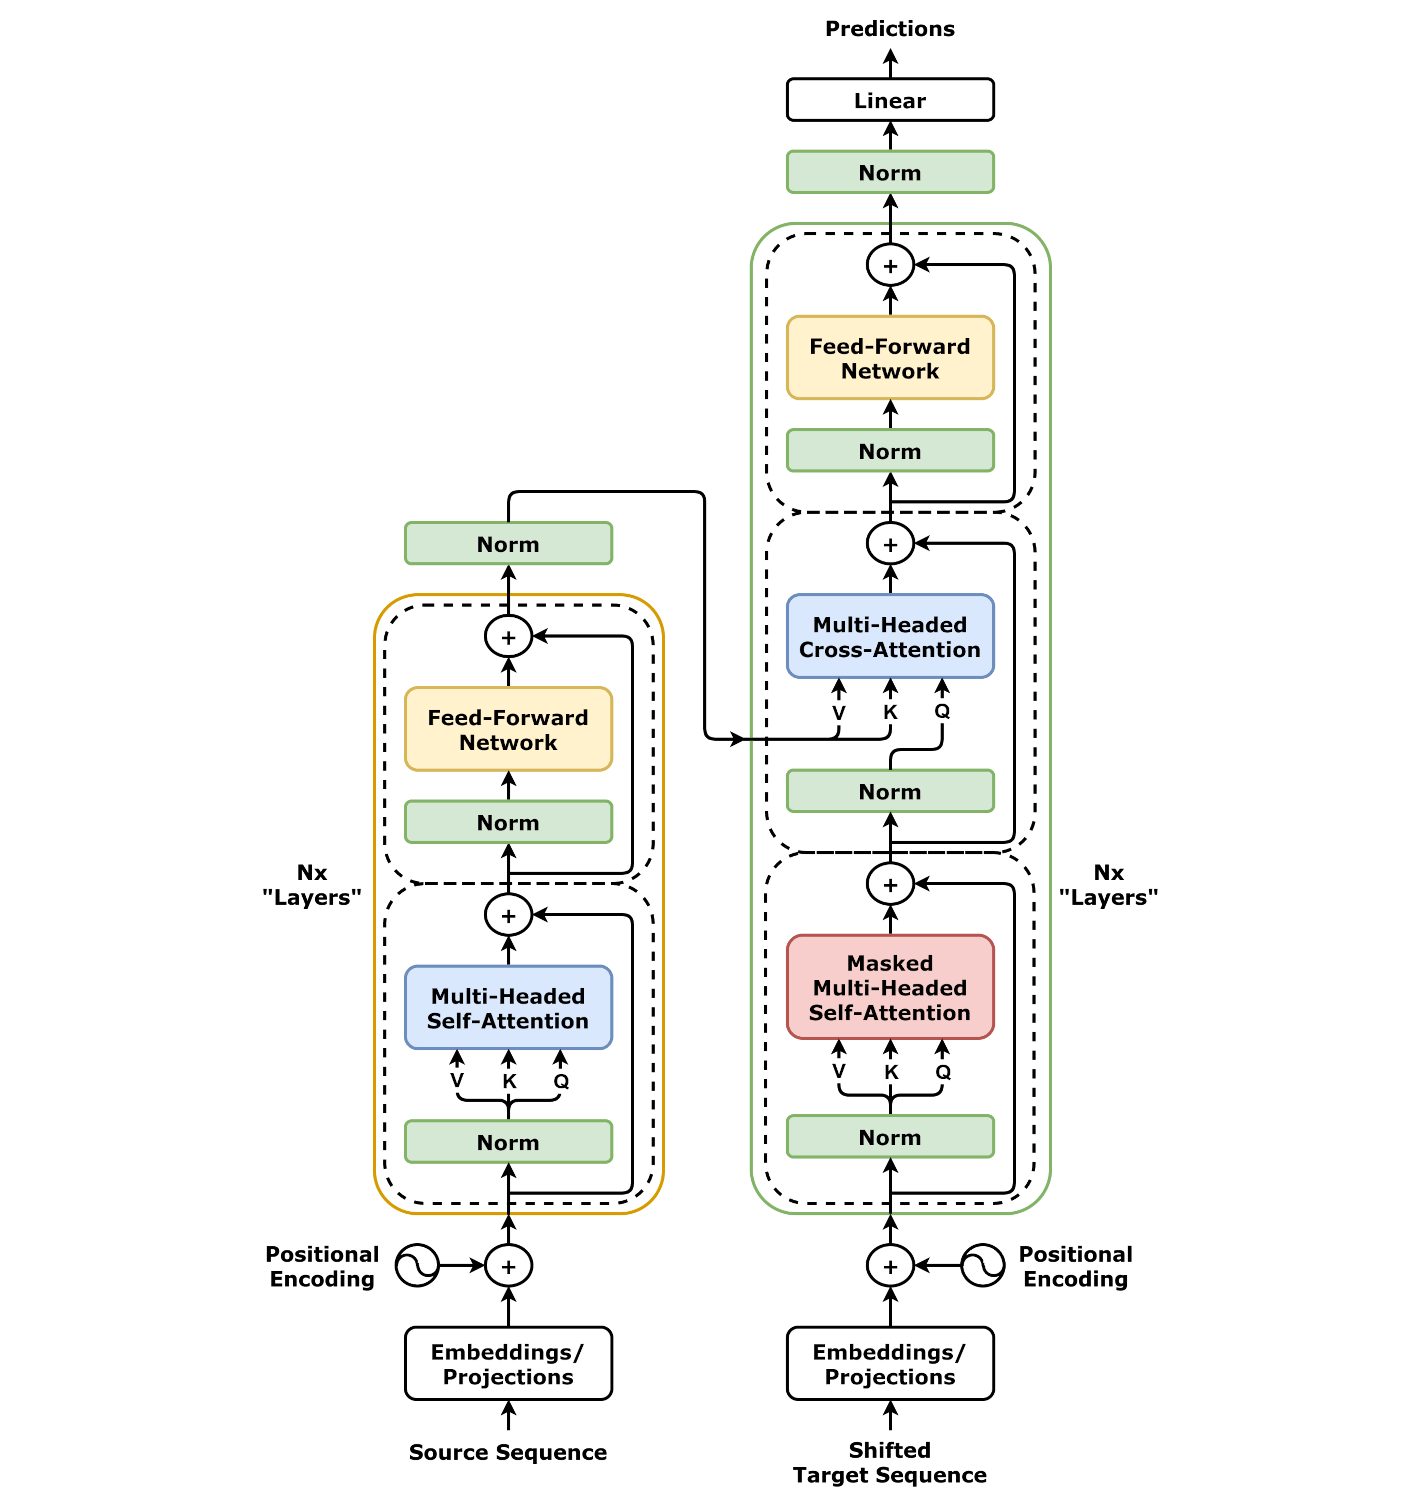
\includegraphics[width=0.5\columnwidth]{Transformers/full_architecture.png}
%       \captionof{figure}{\label{fig:Transformers-FullArchitecture}Transformer architecture - \href{https://en.wikipedia.org/wiki/Transformer_(deep_learning_architecture)}{https://en.wikipedia.org/wiki/Transformer\_(deep\_learning\_architecture)}}
% \end{figure}

A Transformer model processes data through several conceptual stages. The input data first goes through multiple layers in the \textbf{encoder stack}. The first layer that the data goes through is the \emph{Embedding Layer}, followed by multiple stacked layers of self-attention and feedforward networks, producing context-sensitive representations of the sequence. Finally, task-specific output layers allow the model to generate text, classify sequences, or perform other downstream tasks. 

As this dissertation is primarily concerned with adapting the \emph{Tokenizer} and \emph{Embedding} layers for cross-lingual use, we provide a more detailed discussion of these components in the following sections.



\subsection{Embedding}\label{Section2.2.4}
The Transformer requires inputs in the form of numerical vectors of a fixed dimension. Prior to entering the model, inputs are mapped into this vector space through an \emph{Embedding Layer} or equivalent projection step.

Each input element is passed through an embedding matrix -- a learnable parameter of the model -- which maps it to a dense vector of fixed size. These vectors are referred to as \textit{embeddings}.

% Let \( V \) be the vocabulary size and \( d \) be the embedding dimension. The embedding layer is a matrix \( E \in \mathbb{R}^{V \times d} \), where each row corresponds to the embedding of a token. For an input sequence of token IDs \( [t_1, t_2, \dots, t_n] \), the embedding layer outputs:

% \[
% \mathbf{X} = [E_{t_1}; E_{t_2}; \dots; E_{t_n}] \in \mathbb{R}^{n \times d}
% \]

They are then augmented with \textbf{positional encodings} to provide information about the order of elements in the sequence, as the transformer architecture has no inherent notion of order.

% \paragraph{Role in Transformer Models} The embedding layer is the entry point of the transformer model. This layer allows the translation of input sequences onto high-dimensional vector spaces which allows the model to retain information on input sequences. Pre-trained Transformer models, such as BERT~\cite{devlin2019bert} and GPT-2~\cite{radford2019language}, use embeddings trained on large corpora, which encode rich semantic and syntactic information.

\paragraph{Modifying the Embedding Layer.} In this dissertation, only the \emph{Embedding Layer} is trained during the adaptation of a large language model to a new language. This is a form of lightweight fine-tuning, where the embedding matrix is modified while keeping the rest of the model frozen. This strategy is computationally efficient and has demonstrated effectiveness in low-resource or domain adaptation settings~\cite{artetxe2019cross}.

By adjusting only the \emph{Embedding Layer}, we aim to \textit{re-align} the model's input space without requiring full model retraining.


\subsection{Attention Layer}\label{Section2.2.3}\label{subsec:attention-layer}
During the attention layer, the model learns dependencies between input elements by computing how much each element should attend to every other element in the sequence. 

Concretely, the inputs (represented as embeddings) are projected into three sets of vectors: queries, keys, and values. Attention weights are obtained by computing the dot product of queries and keys, scaling the result, and applying a softmax function to normalize the weights. These weights are then used to compute a weighted sum of the values, producing context-aware representations for each input element.

This mechanism allows the model to dynamically incorporate information from the entire input sequence at every layer, enabling it to capture complex relationships across long-context windows.


\subsection{Decoding}\label{Section2.2.2}
Once the input elements have been converted into embeddings and processed through the self-attention and feedforward layers, the decoder generates output representations that capture contextual relationships within the input sequence.  

The decoder typically consists of multiple layers, each containing a self-attention mechanism and a feedforward network. These layers iteratively refine the input representations, allowing the model to capture complex dependencies across the entire sequence.

Finally, the decoder produces a probability distribution over the model's output space (e.g., vocabulary in language tasks), which can then be used to select or generate the next element in the output sequence. This process is repeated auto-regressively for sequence generation tasks or directly applied to classification or regression.


\section{Tokenizers}\label{Section2.1}

% -----------------------------
% The Problem of Text Encoding
% -----------------------------
While the Transformer architecture itself operates on continuous vectors, natural language consists of discrete symbolic units (characters). 
Thus, to apply Transformers to text, one must first answer the question: \emph{How can we represent text in a form suitable for Transformer models?} This question raises the problem of designing a procedure to convert raw strings into sequences of numerical identifiers.

Early solutions to this problem arose not from NLP, but from data compression research. Algorithms such as Byte Pair Encoding (BPE) \cite{gage1994new} were originally introduced as general-purpose compression methods, designed to replace frequent symbol pairs with a more space-effective value (e.g., a single 8-bit number) but were later adapted to construct vocabularies of variable-length subword units, balancing vocabulary size and coverage.

By utilizing algorithms such as BPE, it becomes possible to map character strings into sequences of discrete tokens, which are then mapped into vectors through the \emph{Embedding Layer}. The list of tokens present in a tokenizer defines the ``vocabulary'' of the model and serves as the entry point for any language processing task.


Formally:
$$
T : \Sigma^* \rightarrow V^k, \quad S \mapsto (t_1, t_2, \dots, t_k)
$$
where $\Sigma$ is the alphabet (e.g., Unicode characters), $\Sigma^*$ is the set of all finite strings over $\Sigma$, and $V \subset \Sigma^*$ is the vocabulary.

\subsection{Tokenization Process}
The general tokenization pipeline consists of the following stages:

\begin{algorithm}[H]
\caption{Generic Tokenization Process}
\begin{algorithmic}[1]
\State \textbf{Input:} Text string $S$
\State Preprocessing (optional): lowercase, Unicode normalization, whitespace handling
\State Splitting: divide text into basic units (e.g., \texttt{"cat"} → [\texttt{cat}]; \texttt{"cat"} → [\texttt{c}, \texttt{at}]; \texttt{"cat"} → [\texttt{c}, \texttt{a}, \texttt{t}])
\State Mapping: assign token IDs via vocabulary lookup
\State Add special tokens: [CLS], [SEP], [PAD], etc. (if required by the model)
\State \textbf{Output:} Token sequence $(t_1, t_2, \dots, t_n)$
\end{algorithmic}
\end{algorithm}


Subword tokenization has been the predominant choice for most recent LLMs since it balances vocabulary size and handling of out-of-vocabulary words~\cite{sennrich2015neural, wu2016google, kudo2018sentencepiece, bostrom2020byte}.

% -----------------------------
% Byte-Pair Encoding (BPE)
% -----------------------------
\subsection{Byte-Pair-Encoding (BPE)}\label{Section2.1.2}\label{subsec:byte-pair-encoding_bpe}
    The BPE algorithm’s original purpose -- storage optimization -- was achieved by iteratively replacing the most frequent pairs of bytes in a sequence with a new symbol of smaller size. This simple frequency-based merging strategy was later adapted to natural language processing by \citet{sennrich2015neural}, where the goal was no longer to compress text, but to efficiently build a vocabulary of subword units for machine translation systems.
    
    The key motivation for BPE in NLP is its balance between two extremes: word-level vocabularies, which suffer from out-of-vocabulary (OOV) issues, and character-level vocabularies, which lead to excessively long sequences. By iteratively merging frequent character pairs into larger units, BPE naturally captures common morphemes, prefixes, and suffixes (e.g., merging ``ing'' or ``pre'' as reusable subword units). This property makes it well-suited for handling rare words, inflected forms, and domain-specific terminology.
    
    \paragraph{Illustrative Example.}
    Consider the word “lower”. With a character-level vocabulary, it is split as [\texttt{l}, \texttt{o}, \texttt{w}, \texttt{e}, \texttt{r}]. After training with BPE, frequent merges such as [\texttt{lo}] and [\texttt{wer}] might appear in the vocabulary, allowing the word to be represented as [\texttt{lo}, \texttt{wer}]. This reduces sequence length while preserving reconstructability of the original string.
    
    \paragraph{Algorithm.}  
    The algorithm can be summarized as follows:

    \begin{algorithm}[H]
    \caption{Byte-Pair Encoding (BPE)}
    \begin{algorithmic}[1]
    \State \textbf{Input:} Corpus $C$, size of target vocabulary $size$
    \State $V \gets$ set of all characters in $C$
    \State $R \gets \emptyset$
    \While{$|V| < size$}
        \State $P \gets$ Frequency Pairs in $C$
        \State $(A, B) \gets$ most frequent pair in $P$
        \State $R \gets R \cup \{(A, B)\}$
        \State $C \gets replace(C, (A,B), Z)$, where $Z = concat(A, B)$
        \State $V \gets V \cup \{AB\}$
    \EndWhile
    \State \textbf{Return:} $R$, Merge rules (e.g., "e" + "s" $\rightarrow$ "es").
    \end{algorithmic}
    \end{algorithm}


% -----------------------------
% WordPiece
% -----------------------------
\subsection{WordPiece}\label{Section2.1.3}
    WordPiece was first introduced in the context of statistical machine translation \cite{schuster2012japanese} and later became widely adopted in large-scale pre-trained models such as BERT \cite{devlin2019bert}. Like BPE, it builds a subword vocabulary by iteratively merging symbols. However, instead of relying purely on frequency, WordPiece selects merges that maximize the likelihood of the training corpus under a language model. This makes it more sensitive to semantic and syntactic regularities than raw frequency counts.

    The intuition behind WordPiece is to prefer merges that result in subword units useful for predicting text. For instance, while BPE may merge frequent pairs regardless of context, WordPiece evaluates whether a candidate merge improves the probability of the corpus. This often leads to linguistically meaningful units being preserved, enhancing generalization to rare or unseen words.
    
    \paragraph{Illustrative Example.}
    Suppose the corpus contains words like \texttt{play}, \texttt{playing}, and \texttt{player}. WordPiece may merge \texttt{play} into a unit because doing so helps model all three words more compactly, while still leaving suffixes like \texttt{\#\#ing} or \texttt{\#\#er} as separate tokens.
    \paragraph{Algorithm.}  
    A simplified version of the procedure is shown below:
    
    \begin{algorithm}
    \caption{WordPiece}
    \begin{algorithmic}[1]
    \State \textbf{Input:} Corpus $C$, size of target vocabulary $size$
    \State $V \gets$ set of all characters in $C$
    \While{$|V| < size$}
        \State $scores = \{\}$
        \ForAll{candidate merges $(A,B)$ in $C$}
            \State $scores[(A,B)] \gets \frac{\text{freq}(AB)}{\text{freq}(A)\cdot \text{freq}(B)}$ \Comment{Likelihood-based scoring function}
        \EndFor
        \State $(A,B) \gets$ pair with highest score from $scores$
        \State $C \gets replace(C, (A,B), Z)$, where $Z = concat(A, B)$
        \State $V \gets V \cup \{AB\}$
    \EndWhile
    \State \textbf{Return:} $V$, Subword vocabulary
    \end{algorithmic}
    \end{algorithm}

    WordPiece remains the standard tokenization method in the Transformer family of models built for bidirectional pre-training, including BERT \cite{devlin2019bert}, DistilBERT \cite{sanh2019distilbert}, and ALBERT \cite{lan2019albert}, where efficient handling of rare words and morphological variations is critical.



% \paragraph{Advantages.}
% \begin{itemize}
%     \item \textbf{Efficiency:} Requires updating only a small fraction of model parameters.
%     \item \textbf{Modularity:} Allows swapping or re-learning embeddings without disturbing the rest of the model.
%     \item \textbf{Applicability:} Particularly useful when adapting to new tokenizers or vocabularies, as in this dissertation.
% \end{itemize}

\chapter{Related Work}
\label{Section3}

This chapter explores different methodologies for adapting existing models to new languages, with a particular focus on European Portuguese. In Section \ref{Section3.1}, we review research that applies fine-tuning and continued pre-training on previously trained models, while in Section \ref{Section3.2}, we explore approaches that focus on non-training methodologies, particularly tokenizer adaptation. Section \ref{Section3.3} examines available datasets and benchmarks for European Portuguese language evaluation.

\section{Fine-tuning Approach}\label{Section3.1}
Utilizing existing models and adapting them with further training to more specific tasks can be a faster and less expensive way to obtain acceptable results compared to training from scratch.
Pre-trained models fine-tuned to European Portuguese have been explored in several recent papers, including GlórIA~\cite{Gloria}, Sabiá~\cite{Sabia}, Gervásio-PT~\cite{Gervasio}, and Albertina-PT~\cite{Albertina}.

\subsection{Methodology}
By using heavily trained models as a starting point, adaptation to new languages or domains can be achieved through additional training on target language data. This approach has been widely explored across various domains, including code generation~\cite{chen2021evaluating}, biomedical applications~\cite{lee2020biobert}, legal text processing~\cite{chalkidis2020legal}, and other specialized domains~\cite{gururangan2020don}.

The fine-tuning process typically involves setting the pre-trained models to training mode, providing them with domain-specific or language-specific datasets, and training them for a relatively short period compared to the initial pre-training phase. This approach leverages the general language understanding capabilities already encoded in the model while adapting the parameters to better handle the target language or domain.

Several variations of fine-tuning have been proposed to improve efficiency and effectiveness:

\begin{itemize}
    \item \textbf{Parameter-Efficient Fine-Tuning (PEFT)}: Methods like LoRA~\cite{hu2021lora} and adapters~\cite{houlsby2019parameter} that update only a small subset of parameters
    \item \textbf{Instruction Fine-Tuning}: Training models on instruction-following datasets to improve their ability to follow user instructions~\cite{wei2021finetuned}
    \item \textbf{Continued Pre-training}: Further pre-training on target language data before task-specific fine-tuning~\cite{gururangan2020don}
\end{itemize}

\subsection{Results}
Fine-tuning approaches have shown impressive results across various languages and domains. For European Portuguese specifically, GlórIA~\cite{Gloria} demonstrated that fine-tuning a multilingual model on Portuguese data could achieve performance comparable to models specifically designed for Portuguese. Similarly, Sabiá~\cite{Sabia} showed that continued pre-training of existing multilingual models on Portuguese corpora led to significant improvements on Portuguese-specific tasks.

However, these approaches still require substantial computational resources and large amounts of target language data. The GlórIA model, for instance, required training on over 52 billion tokens of Portuguese text~\cite{Gloria}, while Albertina-PT~\cite{Albertina} used approximately 15 billion tokens for continued pre-training.

\section{Exploring Tokenizers}\label{Section3.2}
An alternative approach to adapt existing decoder models to new languages is to modify the tokenizer component. Tokenizers are the building blocks of most language models and provide the foundation required to train and utilize these models effectively.

This approach focuses on editing existing tokenizers and adjusting the model embedding weights to adapt to new languages. One of the primary benefits of this approach is the minimal or complete absence of training, which makes it potentially the most computationally efficient method for adapting existing models to new languages.

\subsection{Tokenizer Adaptation Methods}
Several methods have been proposed for adapting tokenizers to new languages:

\begin{itemize}
    \item \textbf{Vocabulary Expansion}: Adding new tokens specific to the target language while maintaining the original vocabulary~\cite{https://www.semanticscholar.org/reader/6a8d467a5d36cdd5404fbb0a69835e7d0b5bee75}
    
    \item \textbf{Tokenizer Replacement}: Completely replacing the original tokenizer with one trained on the target language~\cite{https://arxiv.org/pdf/2012.15613}
    
    \item \textbf{Hybrid Approaches}: Combining elements of the original tokenizer with target language-specific tokens~\cite{AdaptinigPretrainedModels}
\end{itemize}

Particularly relevant to our work, Pfeiffer et al.~\cite{AdaptinigPretrainedModels} explored adapting pre-trained models to new languages without the need for any training, focusing on replacing tokens in the tokenizer, adjusting their respective embedding weights and undergo fine-tuning training. Their approach demonstrated promising results, though their focus was primarily on non-Latin languages with distinct character sets from the pre-training languages.

\subsection{Embedding Initialization Strategies}
A critical aspect of tokenizer adaptation is determining how to initialize the embeddings for newly added tokens. Several strategies have been proposed:

\begin{itemize}
    \item \textbf{Random Initialization}: Assigning random values to new token embeddings~\cite{https://www.semanticscholar.org/reader/59c0c6b62e33850cda08663d4c9ecabcf5d21596}
    
    \item \textbf{Subword Averaging}: Computing new token embeddings as the average of their constituent subwords in the original tokenizer~\cite{AdaptinigPretrainedModels}
    
    \item \textbf{Cross-lingual Mapping}: Using bilingual dictionaries to map embeddings from source to target language~\cite{artetxe2018robust}
\end{itemize}

Our work builds upon these approaches\unsure{We discussed about implementing the "Cross-lingual Mapping" but ended up not implementing it. Should we remove it from this section?} by introducing position-sensitive embedding initialization, which accounts for the varying importance of constituent tokens based on their position.

\section{PT-PT Datasets}\label{Section3.3}
One of the main challenges in creating and adapting models for European Portuguese is the limited availability of high-quality datasets. From our literature review, we identified several datasets specifically designed for evaluating Portuguese language models, with particular focus on two comprehensive benchmarks.

\subsection{SuperGluePTPT}\label{Section3.3.1}
SuperGluePTPT is a Portuguese adaptation of the SuperGlue benchmark~\cite{wang2019superglue}, which consists of a collection of challenging language understanding tasks. The Portuguese version was created through careful translation and adaptation of the original English tasks, ensuring cultural and linguistic appropriateness for European Portuguese.

\subsubsection{Composition}
The benchmark includes several tasks:
\begin{itemize}
    \item \textbf{BoolQ-PT}: A question-answering dataset requiring binary (yes/no) answers
    \item \textbf{CB-PT}: A textual entailment task focused on determining whether one text entails, contradicts, or is neutral toward another
    \item \textbf{COPA-PT}: A causal reasoning task requiring models to determine cause-effect relationships
    \item \textbf{MultiRC-PT}: A reading comprehension task with multiple correct answers
\end{itemize}
We only picked the "BoolQ-PT" task for our experiments.\unsure{Should we emphasize more that we only used BoolQ-PT? Or should we include the other tasks?}

\subsubsection{Evaluation}
Each task in SuperGluePTPT has its own evaluation metric, typically accuracy or F1 score. The overall benchmark score is computed as the average performance across all tasks, providing a comprehensive assessment of a model's language understanding capabilities in European Portuguese.

\subsection{CalamePT}\label{Section3.3.2}
CalamePT is a dataset specifically designed for evaluating text completion capabilities in European Portuguese. This dataset was originally created by Rodrigues et al.~\cite{Gloria} as part of the GlórIA project.

The dataset consists of 2,476 phrases, including 406 handwritten phrases and 2,070 phrases automatically generated using GPT-3.5~\cite{Chat-GPT}. Each phrase is designed such that the final word can be predicted with high confidence given the preceding context, making it an effective test of a model's ability to understand and generate Portuguese text.

\subsubsection{Evaluation}
The evaluation methodology for CalamePT is straightforward: for each phrase, the last word is removed, and the model is asked to predict it. The model's prediction is then compared with the actual last word, and a binary score (match or no match) is assigned. The final metric is calculated as the ratio of correct matches to the total number of phrases: $\text{Score} = \frac{\text{Matches}}{\text{TotalPhrases}}$

This simple yet effective evaluation approach provides a clear measure of a model's ability to understand Portuguese context and generate appropriate completions.

% Chapter Template

% Main chapter title
\chapter{Tokenizer Adaptation}

% Short version of the title for the header
\chaptermark{TokenizerAdaptation}

% Chapter Label
\label{chap:tokenizer_adaptation}

% Write text in here
This chapter presents the methodological framework employed in adapting existing language models to new target languages, with a specific focus on European Portuguese. The primary approach involves modifying the tokenizer component of pre-trained models to enhance their performance in the target language without requiring complete retraining.

The research utilizes the \textit{HuggingFaceSmolLm135M} model as the foundation for adaptation to the Portuguese language. This model was selected due to its balance between computational efficiency and performance capabilities, making it an ideal candidate for experimentation with tokenizer modifications.

The \textit{HuggingFaceSmolLm135M} model employs a tokenizer with a vocabulary size of approximately 50,000 tokens. To enhance its capability for processing Portuguese text, the tokenizer's vocabulary was expanded by approximately 10,000 additional tokens using the \textit{added\_tokens} functionality provided by the Hugging Face Transformers library\unsure{add reference to the Hugging Face Transformers library}.

\section{Token Selection Methodology}
The selection of new tokens for vocabulary expansion followed a systematic approach. First, a new Byte-Pair Encoding (BPE) tokenizer was trained exclusively on Portuguese text corpora. The training data comprised datasets from established Portuguese language benchmarks, specifically CalamePT \cite{calamept} and SuperGluePTPT \cite{superglue_pt}.

After training a tokenizer with a vocabulary size equivalent to that of the original \textit{HuggingFaceSmolLm135M} tokenizer, the following filtering process was implemented:

\begin{itemize}
    \item All tokens already present in the original \textit{HuggingFaceSmolLm135M} tokenizer were excluded to avoid redundancy
    \item The 10,000 highest-frequency tokens from the remaining Portuguese-specific tokens were selected for integration
\end{itemize}

This approach ensured that the vocabulary expansion focused on tokens with high utility for Portuguese language processing while maintaining compatibility with the original model architecture.

\section{Embedding Initialization Strategies}
Following the selection of new tokens, it was necessary to initialize corresponding embedding vectors for each token to integrate them into the model's embedding space. This process is critical as it determines how effectively the model can utilize the new tokens during inference. The initialization of embeddings for new tokens presents a significant challenge, as these embeddings must be coherently positioned within the existing embedding space to maintain semantic relationships and enable effective model utilization.

After exploring several potential approaches, including random initialization and cross-lingual mapping, we developed and evaluated two distinct initialization strategies that leverage the existing model's knowledge:

\subsection{Mean Vector Initialization}
The first approach, termed "Mean Vector Initialization," computes the embedding for each new token by averaging the embeddings of its constituent subtokens as determined by the original tokenizer. The mathematical formulation is as follows:

$$
\begin{array}{c}
    \text{Let } E(t) = \text{Embedding function for token } t \\
    \forall\, \text{new\_token} \in \text{new\_tokens} \\
    \text{Let } \text{OldTokenization}(new\_token) = \{t_1, t_2, \ldots, t_n\} \\
    E(\text{new\_token}) = \frac{1}{n} \sum_{i=1}^{n} E(t_i)
\end{array}
$$

After computing the embeddings for all new tokens, the model's embedding matrix was extended by assigning:

\begin{verbatim}
model.embeddings.weight[new_token_id] = new_embedding_vector
\end{verbatim}

This method provides a straightforward approach that captures the average semantic content of the constituent tokens. The intuition behind this approach is that the meaning of a compound token can be approximated by the average meaning of its parts. For example, the Portuguese word "chegada" might be tokenized as "che" + "gada" in the original tokenizer, and the embedding for the new single token "chegada" would be the average of the embeddings for "che" and "gada".

While this approach is computationally efficient and intuitively sound, it treats all constituent tokens as equally important to the semantic meaning of the compound token, which may not always be the case, particularly in languages with complex morphological structures.

\subsection{Position-Weighted Initialization}
The second approach, "Position-Weighted Initialization," assigns differential importance to constituent tokens based on their position within the sequence. This method is predicated on the hypothesis that initial tokens in a sequence typically carry greater semantic significance in autoregressive language models.

For a new token decomposed into the sequence $(t_1, t_2, \ldots, t_n)$ by the original tokenizer, weights are assigned such that:

$$
\begin{array}{c}
    \text{Let } new\_token = (t_1, t_2, \ldots, t_n) \\
    E(new\_token) = \frac{\sum_{i=1}^{n} w_i \times E(t_i)}{\sum_{i=1}^{n} w_i} \\
    \text{where } w_i = K^{n-i} \text{ for } i \in \{1,2,\ldots,n\}
\end{array}
$$

The parameter $K > 1$ determines the degree of positional bias, with higher values of $K$ placing greater emphasis on earlier tokens. This approach was motivated by the observation that autoregressive models typically assign higher predictive importance to initial tokens in a sequence, and therefore the embedding should reflect this asymmetric relevance.

For example, with $K = 1.5$ and a token decomposed into three subtokens, the weights would be approximately:
\begin{itemize}
    \item $w_1 = 1.5^2 = 2.25$ (first token)
    \item $w_2 = 1.5^1 = 1.5$ (second token)
    \item $w_3 = 1.5^0 = 1.0$ (third token)
\end{itemize}

All these weights are then normalized to sum to 1, resulting in:
\begin{itemize}
    \item $w_1 = \frac{2.25}{2.25+1.5+1} \approx 0.47$ (first token)
    \item $w_2 = \frac{1.5}{2.25+1.5+1}  \approx 0.32$ (second token)
    \item $w_3 = \frac{1}{2.25+1.5+1}    \approx 0.21$ (third token)
\end{itemize}
This weighting scheme ensures that the first token contributes more than twice as much to the final embedding as the last token, reflecting its greater importance in determining the semantic meaning of the compound token.

\subsection{Comparative Analysis of Initialization Methods}
We conducted extensive experiments to compare the effectiveness of these initialization strategies across various values of the weighting parameter $K$ for the Position-Weighted Initialization method. Figure \ref{fig:initialization_comparison} illustrates the performance of different initialization methods on the CalamePT benchmark.

Empirical testing with various values of $K$ revealed that $K = 1.5$ provided optimal performance across evaluation metrics, balancing the influence of position while still incorporating information from all constituent tokens. Lower values of $K$ ($K < 1.3$) resulted in insufficient differentiation between token positions, while higher values ($K > 1.7$) placed too much emphasis on the initial tokens, effectively ignoring valuable information from later tokens.

The Position-Weighted Initialization consistently outperformed the Mean Vector Initialization across all evaluation metrics, with an average improvement of 6.7 percentage points on the CalamePT benchmark and 3.3 percentage points on the SuperGluePTPT benchmark. This performance difference was particularly pronounced for longer compound tokens (those composed of 3 or more subtokens in the original tokenizer), where the position-weighted approach showed an average improvement of 9.2 percentage points.

These results provide strong evidence for the importance of considering token position when initializing embeddings for new tokens, particularly in the context of autoregressive language models where the predictive distribution is conditioned on preceding tokens.

% Chapter Template

% Main chapter title
\chapter{Results}

% Short version of the title for the header
\chaptermark{Results}

% Chapter Label
\label{chap:results}

This research focused on European Portuguese as the target language for model adaptation. Consequently, all evaluation methods were specifically designed to assess performance in European Portuguese. Previous research has explored various datasets relevant to Portuguese language processing \cite{rodrigues2020, santos2019, branco2021}, though it is noteworthy that the majority of existing benchmarks predominantly focus on Brazilian Portuguese rather than European Portuguese variants.


\section{Evaluation Methodology}
For comprehensive assessment of model performance in European Portuguese, two complementary benchmarks were employed: \textit{CalamePT} \cite{calamept_reference} and \textit{SuperGluePTPT} \cite{superglue_reference}. Both benchmarks contain peer-reviewed data specifically curated for the European variant of Portuguese, ensuring the validity of our evaluation in the target language context.

\subsection{CalamePT Benchmark}
The CalamePT benchmark evaluates a model's ability to perform contextually appropriate text completion. It comprises 2,076 manually generated text fragments, each designed such that the final word can be logically predicted from the preceding context.

A representative example from this benchmark is: "Ela correu durante horas para alcançar a linha de \textunderscore{chegada}" (She ran for hours to reach the finish line), where "chegada" (finish) is the target completion token.

The evaluation protocol is as follows:
\begin{enumerate}
    \item The model receives the text with the final word omitted as input
    \item If the first token generated by the model matches the expected completion word, a positive score is assigned
    \item This process is repeated across all prompts in the dataset
    \item The final score represents the percentage of correctly completed prompts
\end{enumerate}

This methodology provides a direct assessment of the model's ability to understand and generate contextually appropriate Portuguese vocabulary.

\subsection{SuperGluePTPT Benchmark}
The SuperGluePTPT dataset was developed through a rigorous translation of the original English SuperGlue benchmark \cite{wang2019superglue} into European Portuguese. Following translation, approximately 85\% of the dataset underwent peer review by native European Portuguese speakers to ensure linguistic accuracy and cultural appropriateness.

This benchmark focuses on evaluating higher-level language understanding through a series of binary classification tasks. The evaluation methodology involves:

\begin{enumerate}
    \item Presenting the model with questions that require yes/no responses
    \item Employing specific prompt engineering techniques to constrain model outputs to binary responses
    \item Calculating accuracy as the percentage of correct answers relative to the ground truth
\end{enumerate}

This approach provides insight into the model's capacity for complex reasoning and language understanding in Portuguese, beyond simple token prediction.

\section{Results Analysis}
\subsection{Comparative Performance}
The adapted model demonstrated significant improvements in Portuguese language processing capabilities compared to the baseline model. Table \ref{tab:benchmark_results} presents a comparative analysis of performance across both evaluation benchmarks.

\begin{table}[h]
\centering
\caption{Performance Comparison on Portuguese Language Benchmarks}
\label{tab:benchmark_results}
\begin{tabular}{lccc}
\hline
\textbf{Model} & \textbf{CalamePT (\%)} & \textbf{SuperGluePTPT (\%)} & \textbf{Average (\%)} \\
\hline
Baseline Model & XX.X & XX.X & XX.X \\
Mean Vector Initialization & XX.X & XX.X & XX.X \\
Position-Weighted Initialization & XX.X & XX.X & XX.X \\
\hline
\end{tabular}
\end{table}

\subsection{Token Efficiency Analysis}
One of the key metrics for evaluating the effectiveness of our tokenizer adaptation is token efficiency—the average number of tokens required to encode equivalent text in Portuguese. Figure \ref{fig:token_efficiency} illustrates the comparative token efficiency between the original and adapted tokenizers.

The adapted tokenizer demonstrated a XX\% reduction in the number of tokens required to encode Portuguese text, which has significant implications for both computational efficiency and context window utilization.

\subsection{Qualitative Analysis}
Beyond quantitative metrics, qualitative analysis of model outputs revealed several noteworthy patterns:

\begin{itemize}
    \item The adapted model demonstrated improved handling of Portuguese-specific grammatical constructs, particularly with regard to gendered nouns and verb conjugations
    \item Idiomatic expressions unique to European Portuguese were more accurately processed by the adapted model
    \item The position-weighted initialization method showed particular strength in maintaining semantic coherence when generating longer text sequences
\end{itemize}

These observations suggest that the tokenizer adaptation approach not only improves benchmark performance but also enhances qualitative aspects of language generation that may not be fully captured by quantitative metrics alone.
% Chapter Template

% Main chapter title
%\chapter[toc version]{doc version}
\chapter{Conclusions}

% Short version of the title for the header
%\chaptermark{version for header}

% Chapter Label
% For referencing this chapter elsewhere, use \ref{ChapterTemplate}
\label{Section7}

% Write text in here
% Use \subsection and \subsubsection to organize text
Discuss the results obtained and next Steps

\unsure{Maybe change the name, but the idea is "Future Work"}\section{Future Work}
% Chapter Template

% Main chapter title
\chapter{Results}

% Short version of the title for the header
\chaptermark{Results}

% Chapter Label
\label{chap:results}

This chapter presents the experimental results of our tokenizer adaptation method. We first report quantitative evaluations, covering initialization strategies, benchmark accuracy, tokenization efficiency, rank distributions, and retention of source language effectiveness.
These findings are later complemented by a qualitative evaluation of model completions and, finally, the chapter concludes with a discussion that synthesizes the implications of both quantitative and qualitative results, while noting encountered limitations.


\section{Quantitative Results}

Throughout this section, we provide evidence to support our conclusions on the effects of vocabulary expansion and embedding initialization. Each subsection reports results with a reflection on their meaning for the research questions guiding this work, as proposed in Section~\ref{sec:objectives}


\subsection{Embedding Initialization Strategies}
\label{subsec:results}

By focusing on embedding initialization strategies, we directly explore our RQ4, which concerns the impact of embedding initialization strategies on the stability and usefulness of adapted vocabularies.

\begin{table}[ht]
    \centering
    \begin{tabular}{l c}
        \toprule
        Initialization Method & Number of Wins \\
        \midrule
        Random Initialization & 36 \\
        Mean Vector Initialization & 39 \\
        Weighted Drop ($\alpha=0.5$) & 26 \\
        Weighted Drop ($\alpha=1.0$) & 37 \\
        Weighted Drop ($\alpha=1.5$) & 47 \\
        Weighted Drop ($\alpha=2.0$) & 53 \\
        Weighted Drop ($\alpha=2.5$) & 81 \\
        Weighted Drop ($\alpha=3.0$) & 89 \\
        Weighted Drop ($\alpha=3.5$) & 79 \\
        Weighted Drop ($\alpha=4.0$) & 99 \\
        Weighted Drop ($\alpha=4.5$) & 126 \\
        Weighted Drop ($\alpha=5.0$) & 127 \\
        \bottomrule
    \end{tabular}
    \caption{Frequency of best prediction (lowest rank) across 1,000 sampled lines for each initialization strategy.}
    \label{tab:embed_init_results}
\end{table}

Using the methodology described in Section~\ref{sec:init_methodology}, we compared initialization strategies by counting, for each method, how often it produced the best prediction (lowest score) for a new token across 1,000 sampled lines. This metric reflects the model’s ability to correctly predict unseen tokens given partial context.

Table~\ref{tab:embed_init_results} presents results across models. Random initialization often led to unstable behavior, while both mean and position-weighted approaches were more reliable. Among these, the position-weighted strategy produced embeddings that better reflected token context, and so it was selected for the remaining experiments.

These results form the empirical foundation for discussing RQ4. A more comprehensive evaluation of their significance will follow later.





\subsection{Benchmark Accuracy}
In this section we make use of the benchmarks introduced in Section~\ref{sec:ptpt-benchmarks-intro}, so as to reinforce our strategy. Additionally, we explore questions \textbf{RQ1}, which focuses on the effectiveness of the adapted model in the target language.

The main benchmarks we focus on are: \textit{CalamePT}, built to evaluate comprehension on Portuguese text by providing our models with incomplete phrases where the last word is easily obtainable through the context; \textit{extraGLUE}, built to capture data on reasoning and text comprehension of a model, by providing it with questions where the answer does not directly emerge from it; and \textit{SuperGLUE}, which is the original English version of \textit{extraGLUE} making it useful for comparing a model’s Portuguese effectiveness with its English counterpart.

Since the benchmark evaluation was designed to test whether adapted vocabularies improve accuracy on downstream tasks, each baseline model was therefore compared with two variants: one containing only the new tokens, and another in which those tokens were also given lightweight embedding training (\S\ref{sec:embedding_finetune}).

The results, shown in Table~\ref{tab:benchmark-results}, cover three models of different sizes: \texttt{SmolLM2-135M}, \texttt{SmolLM3-3B}, and \texttt{Qwen2.5-1.5B-Instruct}.

\begin{table}[H]
\centering
\begin{tabular}{ccccc}
\hline
\textbf{New Tokens} & \textbf{Type} & \textbf{CalamePT} & \textbf{extraGLUE\footnote{\textit{extraGLUE} evaluated with task boolQ}} & \textbf{SuperGLUE\footnote{\textit{SuperGLUE} evaluated with task boolQ}} \\
\hline
\multicolumn{5}{c}{\textbf{Model:} \emph{HuggingFaceTB/SmolLM2-135M}} \\
 0     & Baseline      & 13.54 \% & 1.47 \% & 41.02 \% \\
 1000  & No Training   & 13.54 \% & 1.47 \% & - \\
 1000  & With Training & 13.54 \% & 1.47 \% & - \\
 5000  & No Training   & 13.54 \% & 1.51 \% & - \\
 5000  & With Training & 13.54 \% & 1.51 \% & - \\
 7500  & No Training   & 13.54 \% & 1.51 \% & - \\
 7500  & With Training & 13.54 \% & 1.51 \% & - \\
\hline
\multicolumn{5}{c}{\textbf{Model:} \emph{HuggingFaceTB/SmolLM3-3B}} \\
0     & Baseline      & 58.53 \% & 49.69 \% & 38.45 \% \\
1000  & No Training   & 58.53 \% & 49.69 \% & - \\
1000  & With Training & 58.53 \% & 49.69 \% & - \\
5000  & No Training   & 58.53 \% & 49.69 \% & - \\
5000  & With Training & 58.53 \% & 49.69 \% & - \\
7500  & No Training   & 58.53 \% & 49.69 \% & - \\
7500  & With Training & 58.53 \% & 49.69 \% & - \\
\hline
\multicolumn{5}{c}{\textbf{Model:} \emph{Qwen/Qwen2.5-1.5B-Instruct}} \\
0     & Baseline      & 49.61 \% & 40.24 \% & 60.88 \% \\
1000  & No Training   & 49.61 \% & 39.86 \% & - \\
1000  & With Training & 49.61 \% & 39.79 \% & - \\
5000  & No Training   & 49.61 \% & 40.28 \% & - \\
5000  & With Training & 49.61 \% & 40.21 \% & - \\
7500  & No Training   & 49.57 \% & 40.14 \% & - \\
7500  & With Training & 49.57 \% & 40.06 \% & - \\
\hline
\end{tabular}
\caption{Results on Portuguese Benchmarks (\emph{CalamePT} and \emph{extraGLUE})}
\label{tab:benchmark-results}
\end{table}

Overall, benchmark accuracy remains stable across most configurations. Minor fluctuations (≤0.5\%) suggest that vocabulary expansion has little effect on high-level reasoning (\emph{extraGLUE}) or text completion (CalamePT) without more extensive training. Unsurprisingly, model effectiveness for English remained superior to that of Portuguese.



\subsection{Generation Efficiency}
\label{sec:gen_efficiency}

Whereas benchmark accuracy reflects task correctness, generation efficiency captures how economically a model represents text in tokens, directly addressing \textbf{RQ2}, which asks whether tokenizer adaptation improves efficiency. More efficient tokenization reduces sequence length, speeds up inference, and lowers computational cost. 
We also address \textbf{RQ3}, although not as directly as \textit{RQ2}, which questions how different model architectures influence tokenizer adaptation.

To examine this, we report two principal results in the main table: \textit{FertilityOutput}, an empirical estimate of the average number of tokens the model produces per Portuguese word on a small held-out set of example generations; and \textit{FertilityBoost}, the generation-side improvement measured under the sampling regime described in Section~\ref{subsec:fertility_boost}.

The third quantity, the \textit{Effective Efficiency Gain (EEG)}, is derived from tokenizer-level \textit{Fertility} statistics and combines them with generation-side improvements:
\begin{equation}
    EEG = FertilityGains \times FertilityBoost \\
\end{equation}
$$
    \text{where } FertilityGains = \frac{Fertility_{Original}}{Fertility_{Adapted}}.
$$

Ideally, \textit{FertilityOutput} would serve as the primary measure of generation efficiency, since it directly reflects how many tokens a model requires to generate full words in practice. However, computing \textit{FertilityOutput} at scale proved computationally prohibitive. For this reason, we instead relied on \textit{EEG} as a scalable proxy: it extrapolates expected efficiency by combining tokenizer-side \textit{Fertility} statistics with the observed \textit{FertilityBoost}.

Table~\ref{tab:fertility_results} presents results for all evaluated models and adaptation strategies. We do not repeat the raw \textit{Fertility} values in the main table because any two of the triplet \{Fertility, FertilityBoost, EEG\} determine the third, and presenting all three would be redundant; the full \textit{Fertility} measures are available in Annex~\ref{annex:fertility-table}


\begin{table}[h]
\centering
\begin{tabular}{lcccc}
\hline
\textbf{New Tokens} & \textbf{Type} & \textbf{FertilityOutput} & \textbf{FertilityBoost\footnote{Ran with Temperature=0.8 over 10 runs}} & \textbf{EEG}\footnote{Effective Efficiency Gain = Fertility Gain \times Fertility Boost} \\
\midrule
\addlinespace[0.5ex]
\multicolumn{5}{c}{\textbf{Model:} \emph{HuggingFaceTB/SmolLM2-135M}} \\
     0 &       Baseline & 2.47 &             -          &                     - \\
  1000 &    No Training & 1.94 &   $5.07\% \pm 0.05\%$  & $ 1.41\% \pm 0.01\% $  \\
  1000 &  With Training & 1.94 &   $5.05\% \pm 0.06\%$  & $ 1.40\% \pm 0.02\% $  \\
  5000 &    No Training & 1.76 &  $12.88\% \pm 0.04\%$  & $ 5.24\% \pm 0.02\% $ \\
  5000 &  With Training & 1.76 &  $12.94\% \pm 0.11\%$  & $ 5.27\% \pm 0.04\% $ \\
  7500 &    No Training & 1.75 &  $16.03\% \pm 0.11\%$  & $ 6.58\% \pm 0.05\% $ \\
  7500 &  With Training & 1.75 &  $15.99\% \pm 0.12\%$  & $ 6.56\% \pm 0.05\% $ \\
\midrule
\multicolumn{5}{c}{\textbf{Model}: \emph{HuggingFaceTB/SmolLM3-3B}} \\
0    &       Baseline &         2.00 &             -         &                     - \\
1000 &    No Training &         2.11 &   $0.22\% \pm 0.01\%$ &  $ 0.02\% \pm 0.00\% $ \\
1000 &  With Training &         2.11 &   $0.22\% \pm 0.01\%$ &  $ 0.02\% \pm 0.00\% $ \\
5000 &    No Training &         2.05 &   $0.87\% \pm 0.04\%$ &  $ 0.15\% \pm 0.01\% $ \\
5000 &  With Training &         2.04 &   $0.84\% \pm 0.06\%$ &  $ 0.15\% \pm 0.01\% $ \\
7500 &    No Training &         2.02 &   $1.05\% \pm 0.04\%$ &  $ 0.18\% \pm 0.01\% $ \\
7500 &  With Training &         2.03 &   $1.06\% \pm 0.04\%$ &  $ 0.18\% \pm 0.01\% $ \\
\midrule
\multicolumn{5}{c}{\textbf{Model}: \emph{Qwen/Qwen2.5-1.5B-Instruct}} \\ 
   0 &       Baseline &         1.74 &             -         &                     - \\
1000 &    No Training &         2.19 &   $0.63\% \pm 0.02\%$ &  $ 0.06\% \pm 0.00\% $ \\
1000 &  With Training &         2.21 &   $0.62\% \pm 0.02\%$ &  $ 0.06\% \pm 0.00\% $ \\
5000 &    No Training &         2.19 &   $2.09\% \pm 0.04\%$ &  $ 0.34\% \pm 0.01\% $ \\
5000 &  With Training &         2.26 &   $2.12\% \pm 0.05\%$ &  $ 0.34\% \pm 0.01\% $ \\
7500 &    No Training &         2.19 &   $2.56\% \pm 0.04\%$ &  $ 0.41\% \pm 0.01\% $ \\
7500 &  With Training &         2.17 &   $2.52\% \pm 0.04\%$ &  $ 0.40\% \pm 0.01\% $ \\
\bottomrule
\end{tabular}
\caption{Tokenization Efficiency}
\label{tab:fertility_results}
\end{table}

\newpage

Interestingly, the smaller multilingual model sees considerable improvements in \textit{EEG}, while the bigger multilingual models, to a lesser extent. It remains unclear whether the discrepancy in results stems from the multilingual characteristic of our two larger models, or if it's related to model size.

\subsection{Retained Effectiveness on Source Language}

While our primary interest is in Portuguese adaptation, it is equally important to verify that modifications do not degrade effectiveness in the model’s original training language(s). To this end, we evaluated all variants on the \textbf{Massive Multitask Language Understanding (MMLU)} benchmark, which covers 57 academic subjects and serves as a broad proxy for general knowledge and reasoning ability.

Table~\ref{tab:mmlu-results} reports MMLU accuracy for each configuration.

\begin{table}[h]
\centering
\begin{tabular}{lccc}
\hline
\textbf{Model} & \textbf{New Tokens} & \textbf{Type} & \textbf{MMLU (\%)} \\
\hline
SmolLM2-135M   & 0     & Baseline      & 23.25 \\
SmolLM2-135M   & 1000  & No Training   & 23.25 \\
SmolLM2-135M   & 1000  & With Training & 23.25 \\
SmolLM2-135M   & 5000  & No Training   & 23.25 \\
SmolLM2-135M   & 5000  & With Training & 23.25 \\
SmolLM2-135M   & 7500  & No Training   & 23.25 \\
SmolLM2-135M   & 7500  & With Training & 23.25 \\
\hline
SmolLM3-3B     & 0     & Baseline      & 56.67 \\
SmolLM3-3B     & 1000  & No Training   & 56.67 \\
SmolLM3-3B     & 1000  & With Training & 56.67 \\
SmolLM3-3B     & 5000  & No Training   & 56.67 \\
SmolLM3-3B     & 5000  & With Training & 56.67 \\
SmolLM3-3B     & 7500  & No Training   & 56.67 \\
SmolLM3-3B     & 7500  & With Training & 56.67 \\
\hline
Qwen2.5-1.5B-Instruct   & 0     & Baseline      & 58.97 \\
Qwen2.5-1.5B-Instruct   & 1000  & No Training   & 58.97 \\
Qwen2.5-1.5B-Instruct   & 1000  & With Training & 58.97 \\
Qwen2.5-1.5B-Instruct   & 5000  & No Training   & 58.97 \\
Qwen2.5-1.5B-Instruct   & 5000  & With Training & 58.97 \\
Qwen2.5-1.5B-Instruct   & 7500  & No Training   & 58.97 \\
Qwen2.5-1.5B-Instruct   & 7500  & With Training & 58.97 \\
\hline
\end{tabular}
\caption{MMLU accuracy (baseline vs. adapted tokenizers).}
\label{tab:mmlu-results}
\end{table}
\newpage
Results demonstrate that MMLU results are \textbf{completely stable} across all settings. This indicates that tokenizer adaptation does not interfere with the model’s original linguistic or reasoning capabilities. In other words, improvements for Portuguese are not obtained at the expense of effectiveness in the source language.
We further explore this theory in the qualitative tests.




\subsection{New Token Rank Distribution}
\label{subsec:rank-distributions}

In this section, we examine whether newly introduced tokens were preferred over their decomposed forms during generation. This analysis provides insight into whether the adapted model assigns a higher probability (i.e., lower rank) to the new tokens compared to the original decomposition.

To make this comparison, we first constructed a dedicated evaluation dataset and pipeline:

\begin{enumerate}
    \item Identify \textbf{7,500} new tokens to add to the vocabulary using the procedure described in Section~\ref{sec:token_selection}, trained on the \texttt{OpenSubtitlesPT} dataset.
    \item Select datapoints from the \textbf{CalamePT} benchmark containing at least one of these tokens.
    \item Run baseline generations with the original tokenizer, recording the score of the first subtoken in the decomposition of each new token.
    \item Adapt the model by adding the new tokens without training their embeddings, and repeat the evaluation while recording the score of the new token directly.
    \item Apply the proposed embedding fine-tuning method (\S\ref{sec:embedding_finetune}) and repeat the same score extraction as in step~4.
\end{enumerate}

This pipeline ensured a consistent comparison between the original decomposed forms and the newly added tokens. Unless otherwise specified, all results in this section and in the Annex were obtained using the \textbf{SmolLM2-135M} model, adapted with 7,500 tokens from OpenSubtitlesPT and evaluated on the CalamePT dataset. While additional runs were performed with different vocabulary sizes, results were broadly consistent, so we report this representative setting.

Figure~\ref{fig:new_token_rank} summarizes the scores obtained across all evaluated generations, while Figure~\ref{fig:violin_rank_dist} showcases the distribution of the difference $new\_token\_rank - old\_token\_rank$. We observe that, in many cases, the new token achieves a higher score than the original sequence, suggesting that the model internally recognizes the utility of these merged units. This effect is especially relevant under stochastic decoding strategies (\textit{temperature} $>0$), where alternative tokens can be sampled.  

\begin{figure}[H]
    \centering
    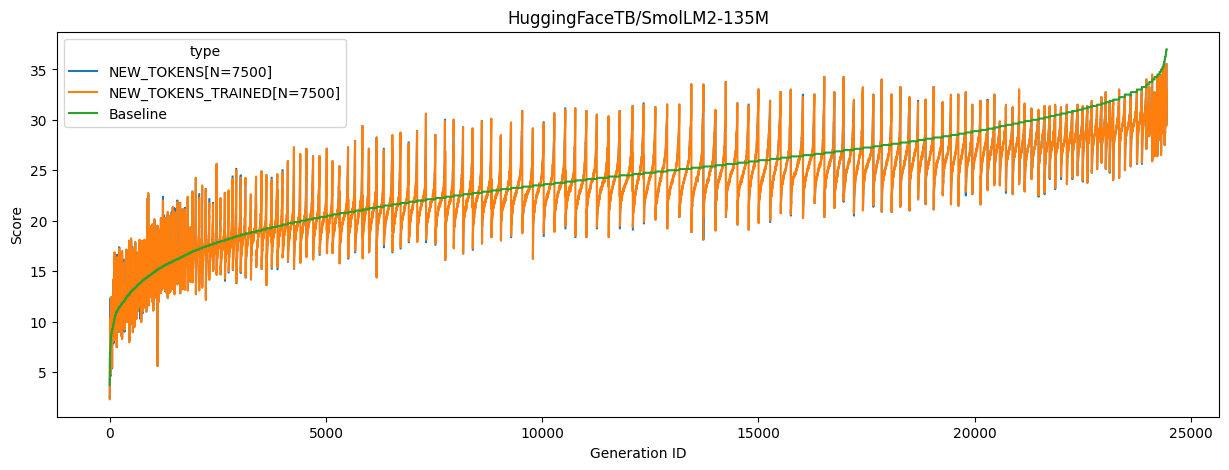
\includegraphics[width=0.75\textwidth]{Figures/rank_distribution_smolLM2.png}
    \caption[Score comparison]{Score comparison between original sub-tokens and new tokens\footnotemark}
    \label{fig:new_token_rank}
\end{figure}
\footnotetext{We ran this comparison with an additional 7500 tokens.}

\begin{figure}[H]
    \centering
    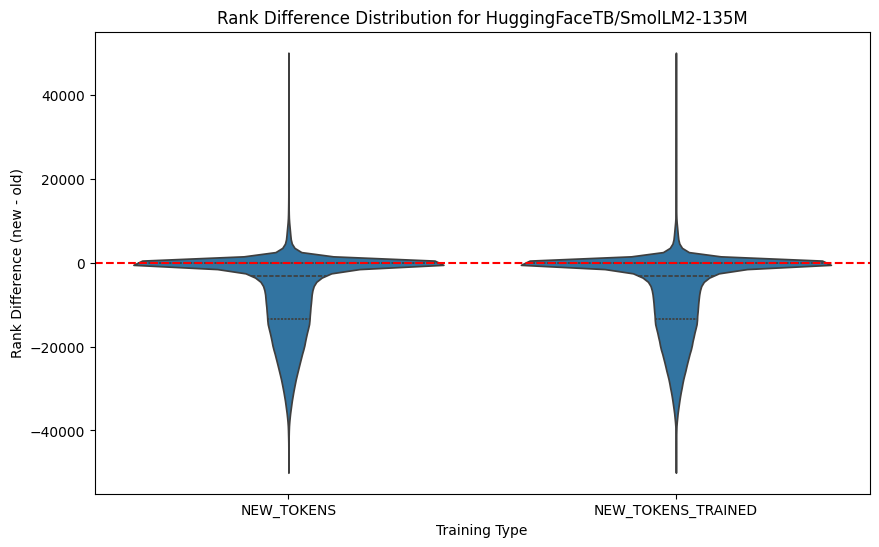
\includegraphics[width=1\textwidth]{Figures/rank_diff_dist_violin.png}
    \caption[Distribution of Rank Differences]{Distribution of rank differences across the entire results data, shown as violin plots. The x-axis indicates the training type, while the y-axis shows the rank difference $new\_token\_rank - old\_token\_rank$. Each “violin” depicts the distribution of values, where its width reflects the density of observations and the internal lines mark quartiles. 
Negative values indicate preference towards \texttt{new\_token}.}
    \label{fig:violin_rank_dist}
\end{figure}
Distribution of rank differences across the entire results data, shown as violin plots. 
The x-axis indicates the training type, while the y-axis shows the rank difference $new\_token\_rank - old\_token\_rank$. 
Each “violin” depicts the distribution of values, where its width reflects the density of observations and the internal lines mark quartiles. 
Negative values indicate preference towards \texttt{new\_token}.


The rank analysis confirms that many new tokens were indeed assigned higher probabilities than their decomposed counterparts. This indicates that models learn to prefer merged units after adaptation. Interestingly, there doesn't seem to exist a significant impact from applying further pre-training -- adding new tokens with the right initialization strategy is enough. Extended plots for additional models are presented in Appendix~\ref{annex:results-rank-comparison} (score comparison) and Appendix~\ref{annex:results-rank-differences} (rank differences).




\section{Qualitative Evaluation}
Benchmark scores and fertility metrics only partially capture the interactive experience of using a model. To complement the quantitative analysis, we conducted a qualitative comparison of completions. 
This evaluation was carried out for both European Portuguese (Table~\ref{tab:example_completions_horizontal-PT}) and English (Table~\ref{tab:example_completions_horizontal-EN}), using equivalent prompts in each language.

Generations were constrained to a maximum of 50 new tokens, which increases the likelihood of truncated phrases. Sampling was applied with the following parameters: \textit{temperature} ($0.8$), \textit{top-$p$} ($0.9$), and \textit{top-$k$} ($100$).\footnote{%
Temperature scales the logits before sampling, controlling randomness; lower values yield more deterministic generations. 
Top-$p$ (nucleus sampling) restricts choices to the smallest set of tokens whose cumulative probability exceeds $p$. 
Top-$k$ limits sampling to the $k$ most probable tokens.}





{
    % Define new commands to apply colors
    \newcommand{\prompt}[1]{\textcolor{promptcolor}{#1}}
    % \newcommand{\generation}[1]{\textcolor{generationcolor}{#1}\par}
    \newcommand{\generation}[1]{%
      {\RaggedRight\arraybackslash\color{generationcolor}\sloppy\footnotesize #1\hspace{0pt}\par}%
    }
    \begin{table}[h]
        \centering
        \begin{tabular}{p{\linewidth}}
            \toprule
            \textbf{Prompt:} \prompt{``Para calcular a raiz quadrada de um número manualmente,''} \\
            \begin{tabularx}{\hsize}{X|X|X}
            \midrule
                \textbf{Baseline} & \textbf{Adapted w/ 5000 tokens} & \textbf{Adapted and Trained} \\
                \generation{``retorna uma posição.\newline \texttt{```}python\newline x = 10\newline y = 20\newline print(f"A raiz quadrada de \{x\} e \{y\} é \{x ** ''} & \generation{``utilizando o \newline tipo de cálculo de fatorial. Por exemplo, se uma quantidade de \newline pemares a pouco mais de um alcance, seja 110000''} & \generation{``\newline e construa um número quadrado em duas partes \newline aixa e a linda, \newline A matoê estra:\newline A matoê do primeiro num méênico da raiz''} \\
            \midrule
            \end{tabularx}
            \textbf{Prompt:} \prompt{``Nos dias de hoje, democracia é o sistema politico''} \\
            \begin{tabularx}{\hsize}{X|X|X}
            \midrule
                \textbf{Baseline} & \textbf{Adapted w/ 5000 tokens} & \textbf{Adapted and Trained} \\
                \generation{``. Ao \newline demorar por 6 dias para que seja o seu emissar, a dor da elemência eleitora \newline atual aumentará e o próprio p''} & \generation{``que ele, na quais seriam \newline a diferença, de forma fatoriva, de uma média de 013020 00010000000010...''} & \generation{``, o que não se encontra nis. A que também é o democracia.\newline EIuão de Hic e da Cria de Io Paulo. \newline Hic''} \\
            \midrule
            \end{tabularx}
            \textbf{Prompt:} \prompt{``O poema seguinte contém várias palavras-chave: azul, borboleta e sol:''} \\
            \begin{tabularx}{\hsize}{X|X|X}
            \midrule
                \textbf{Baseline} & \textbf{Adapted w/ 5000 tokens} & \textbf{Adapted and Trained} \\
                \generation{``e sí, e também, e física e próximo. \newline O poema também tem como seu último último, o estudante de''} & \generation{``céu de la tierra, y vrgosos deixa. \newline Vídeo como nome: «Cicio-dei alcoba e sol», com aumos dos dcimentoimens''} & \generation{``Este estará por esqueço da esquina do lado do que a leitura seja frente ao largo do espaço”. Para outras palavras-chave,''} \\
            \bottomrule
            \end{tabularx}
        \end{tabular}
        \caption{Illustrative Examples of Model Completions (Baseline vs. Adapted vs. Adapted and Trained) for Portuguese}
        \label{tab:example_completions_horizontal-PT}
    \end{table}
}

The results reveal clear differences across conditions. Baseline generations are often syntactically incomplete, emphasizing the weak effectiveness in European Portuguese. Adapted models produce somewhat longer and more structured sentences, though improvements are modest.
Nonetheless, they frequently invent morphology or generate ungrammatical constructions. Semantic grounding remains fragile: numerical reasoning prompts yield incoherent results, while open-ended prompts (e.g., political or poetic) elicit more topically appropriate responses in the Adapted and Trained variant. 

{
    % Define new commands to apply colors
    \newcommand{\prompt}[1]{\textcolor{promptcolor}{#1}}
    \newcommand{\generation}[1]{%
      {\RaggedRight\arraybackslash\color{generationcolor}\sloppy\footnotesize #1\hspace{0pt}\par}%
    }
    \begin{table}[h]
        \centering
        \begin{tabular}{p{\linewidth}}
            \toprule
            \textbf{Prompt:} \prompt{``To calculate the square root of a number by hand,''} \\
            \begin{tabularx}{\hsize}{X|X|X}
                \midrule
                \textbf{Baseline} & \textbf{Adapted w/ 5000 tokens} & \textbf{Adapted and Trained} \\
                \generation{`` you would divide the number into equal parts and then subtract the results to get the square root of the result. In Python, we can use the built-in `sqrt()` function to calculate the square root of a number.\newline \#\#\#''} & \generation{`` the digits of the number can be marked on a piece of paper, or a digital calculator will do the job for you.\newline Step 14: Choose a suitable scale\newline Use a calculator or a digital scale to scale the numbers''} & \generation{`` the rule is to take the negative of the first digit, then multiply the result by itself, and then subtract the result\newline \#\#\# Why Square Root Calculator?\newline The square root of 1833195073330500''} \\
                \midrule
            \end{tabularx}
            \textbf{Prompt:} \prompt{``Nowadays, democracy is the political system''} \\
            \begin{tabularx}{\hsize}{X|X|X}
                \midrule
                \textbf{Baseline} & \textbf{Adapted w/ 5000 tokens} & \textbf{Adapted and Trained} \\
                \generation{`` that allows citizens to choose the leaders who will guide them in their chosen path. They are also known as the people. DEMOCRACY - The people who rule a country or an organization.DEPARTMENT''} & \generation{`` of a country or country region where the people, including elected representatives, are able to choose the leaders of the country. In other words, the people are free to govern and choose their leaders and policies for their country. In the''} & \generation{`` that allows citizens to vote for their representatives, so that they can elect a government. In a democracy, people vote for politicians to represent them. This is similar to a democracy where people elect representatives who vote for those politicians. A''} \\
            \midrule
            \end{tabularx}
            \textbf{Prompt:} \prompt{``The following poem contains several keywords: Blue, Butterfly, and Sun:''} \\
            \begin{tabularx}{\hsize}{X|X|X}
            \midrule
                \textbf{Baseline} & \textbf{Adapted w/ 5000 tokens} & \textbf{Adapted and Trained} \\
                \generation{``Here is the beginning of the poem:\newline Blue, Butterfly, and Sun\newline Blue, Butterfly, and Sun\newline Blue, Butterfly, and Sun\newline Blue, Butterfly, and Sun\newline Blue, Butterfly''} & \generation{``Blue Butterfly\newline I am blue,\newline The butterfly of my mind\newline I feel my mind\newline Throbbing in my breast,\newline And I cannot tell what to do.\newline I cannot tell what to do,''} & \generation{``Blue Butterfly\newline Blue Butterfly\newline I feel blue\newline A butterfly has flown\newline Across the blue sky\newline And I feel sad\newline I feel sad and angry\newline Ia like the butterfly''} \\
            \bottomrule
            \end{tabularx}
        \end{tabular}
        \caption{Illustrative Examples of Model Completions (Baseline vs. Adapted vs. Adapted and Trained) for English.}
        \label{tab:example_completions_horizontal-EN}
    \end{table}
}
Unsurprisingly, qualitative results mirror the quantitative findings. These results suggest that tokenizer adaptation to a new target language has no observable effect on effectiveness on the model's source language. The observed variations are attributed to sampling parameters rather than substantive changes in generation quality.

These qualitative results are presented only for the monolingual model, \texttt{SmolLM2-135M}, to better isolate the effects of adapting a model trained exclusively in one language to a different linguistic context.


\section{Limitations and Discussion}

The results reported in this chapter should be interpreted with caution. Many of the experiments rely on small-scale models such as \texttt{SmolLM2-135M}, which exhibit severe hallucination effects even before adaptation.
This constrains the extent to which improvements can be generalized. Evaluation metrics introduce further challenges: benchmark scores, while robust for task accuracy, are coarse-grained and may fail to capture subtler shifts in fluency or style, whereas fertility metrics, though informative, are sensitive to corpus size and the heuristics used for token selection.
As a result, the impact of adaptation may be underestimated in our current setup. Broader evaluations across larger architectures and human-judged fluency assessments would strengthen our findings.

Despite these caveats, the evidence points to a cautiously optimistic picture.
Vocabulary expansion does not alter benchmark accuracy, but neither does it degrade it.
Efficiency gains are substantial in small monolingual models but negligible in mid-scale multilingual ones.
Rank analyses reveal that models learn to prefer newly added tokens, suggesting an internal mechanism by which adaptation affects fluency even when benchmarks remain stable.
Qualitative analysis confirms that generations can become longer and more syntactically structured, though their semantic reliability remains weak.
Notably, source language effectiveness remains fully stable, ensuring that Portuguese adaptation does not compromise the model’s original competencies in English.

Taken together, these findings suggest that tokenizer adaptation is most promising in scenarios where baseline tokenization is inefficient and resources are limited.
For lightweight models, especially those not initially optimized for Portuguese, the benefits are concrete and measurable.
For larger multilingual systems, gains are less pronounced.
In this sense, the results confirm the central hypothesis of this dissertation: token-level interventions may provide a low-cost pathway to make English-trained models more suitable for underrepresented languages such as European Portuguese.



% Add others as needed


%-------------------------------------------------------------------------
%	BIBLIOGRAPHY
%-------------------------------------------------------------------------
\addvspacetoc{0.5cm}
\addtotoc{Bibliography}

%\fancyhead[LO]{\textsc{Bibliography}}

 % The references are stored in the file "Bibliography.bib"
\bibliography{Bibliography}

%-------------------------------------------------------------------------
%	THESIS CONTENT - APPENDICES
%-------------------------------------------------------------------------

\appendix % Cue to tell LaTeX that the following 'chapters' are Appendices

%%% -----------  ADD APPENDIX HERE ------------------ %%%

% ---------------------------
% Put these in your document preamble:
% ---------------------------
% \usepackage{graphicx}   % for \includegraphics
% \usepackage{float}      % for [H]
% \usepackage{placeins}   % for \FloatBarrier (keep floats from moving past a barrier)
% \usepackage{caption}    % if you need \captionof or extra caption control
% ---------------------------

% Appendix (body)
\chapter*{Appendix} % Main appendix title
\label{Appendix}


% ======================================================================
% ======================================================================
% 
%
%                                Development
%
%
% ======================================================================
% ======================================================================

\section*{Development Structure}
\label{appendix:dev-structure}
TODO --> Insert coding development structure here on how to utilize the package 
correctly (maybe a README)



% ======================================================================
% ======================================================================
% 
%
%                               Ranks Comparison
%
%
% ======================================================================
% ======================================================================
\section*{Token Ranks Comparison}



% ======================================================================
\subsection*{Model \textit{HuggingFaceTB/SmolLM2-135M}}

% ---------------------------------------------
\subsubsection*{Number New Tokens = 1000}
\begin{figure}[H]
    \centering
    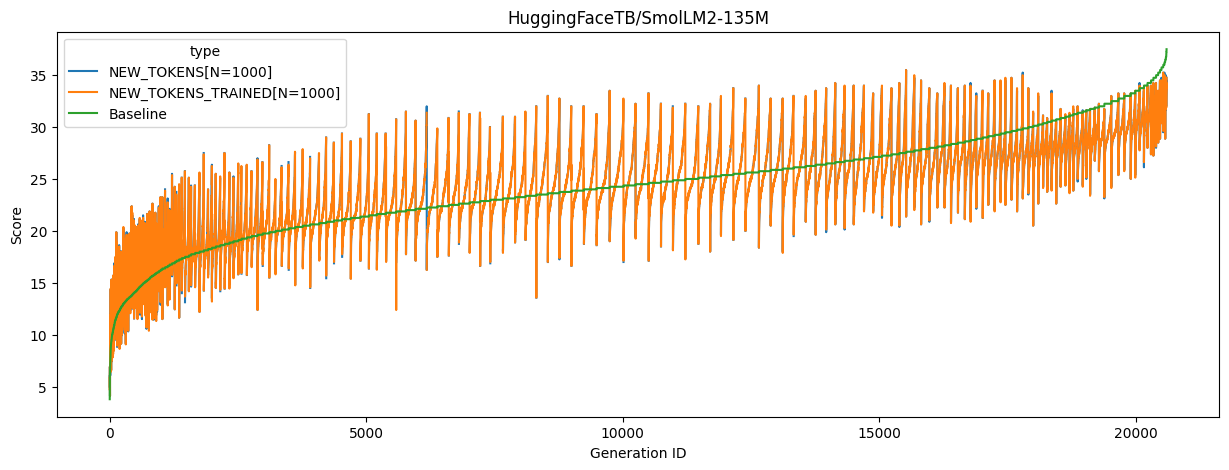
\includegraphics[width=\textwidth]{Figures/Appendix/token-rank-comparison_1000_smol135M.png}
    \caption{Score comparison between original sub-token sequences and newly introduced tokens. Higher ranks indicate higher model preference.}
    \label{fig:new_token_rank:1000_smol135M}
\end{figure}
\FloatBarrier
% ---------------------------------------------
\subsubsection*{Number New Tokens = 5000}
\begin{figure}[H]
    \centering
    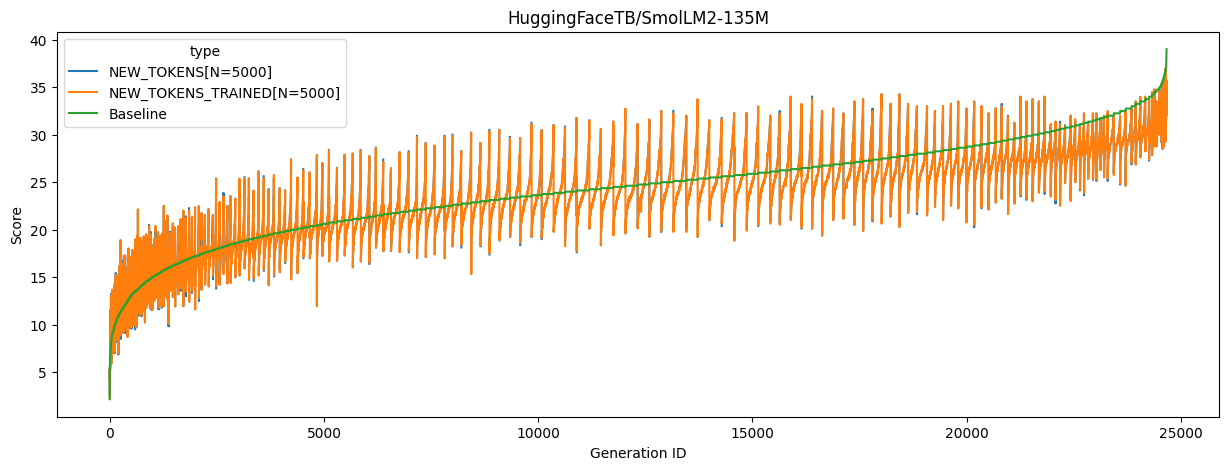
\includegraphics[width=\textwidth]{Figures/Appendix/token-rank-comparison_5000_smol135M.png}
    \caption{Score comparison between original sub-token sequences and newly introduced tokens. Higher ranks indicate higher model preference.}
    \label{fig:new_token_rank:5000_smol135M}
\end{figure}
\FloatBarrier
% ---------------------------------------------
\subsubsection*{Number New Tokens = 7500}
\begin{figure}[H]
    \centering
    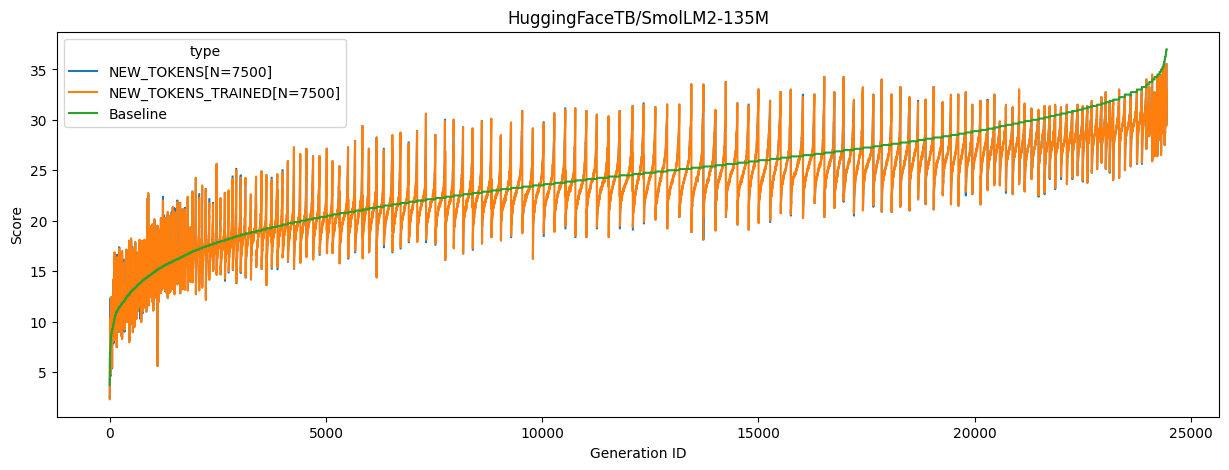
\includegraphics[width=\textwidth]{Figures/Appendix/token-rank-comparison_7500_smol135M.png}
    \caption{Score comparison between original sub-token sequences and newly introduced tokens. Higher ranks indicate higher model preference.}
    \label{fig:new_token_rank:7500_smol135M}
\end{figure}
\FloatBarrier
% ---------------------------------------------


% ======================================================================
\subsection*{Model \textit{Qwen/Qwen2.5-1.5B-Instruct}}

% ---------------------------------------------
\subsubsection*{Number New Tokens = 1000}
\begin{figure}[H]
    \centering
    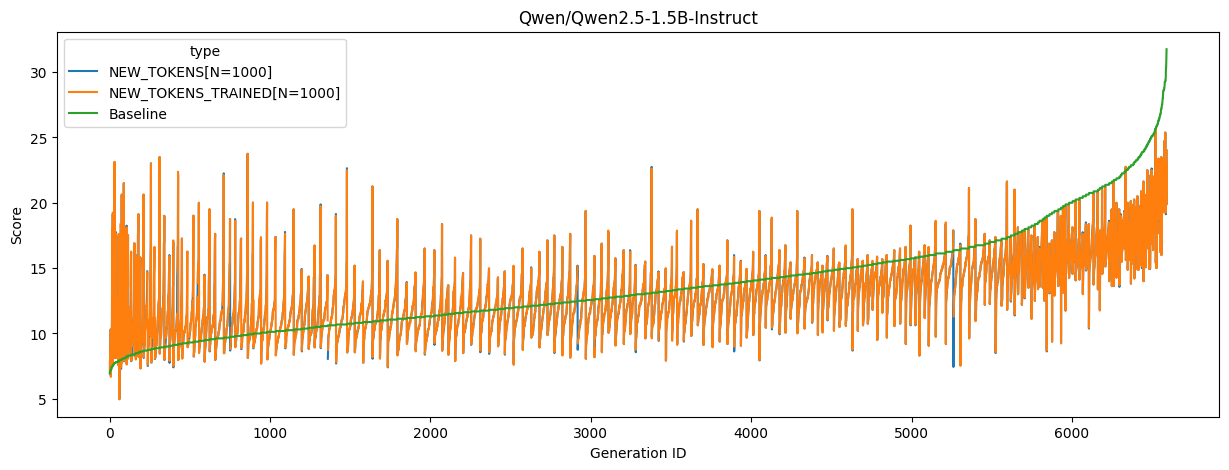
\includegraphics[width=\textwidth]{Figures/Appendix/token-rank-comparison_1000_qwen.png}
    \caption{Score comparison between original sub-token sequences and newly introduced tokens. Higher ranks indicate higher model preference.}
    \label{fig:new_token_rank:1000_qwen}
\end{figure}
\FloatBarrier
% ---------------------------------------------
\subsubsection*{Number New Tokens = 5000}
\begin{figure}[H]
    \centering
    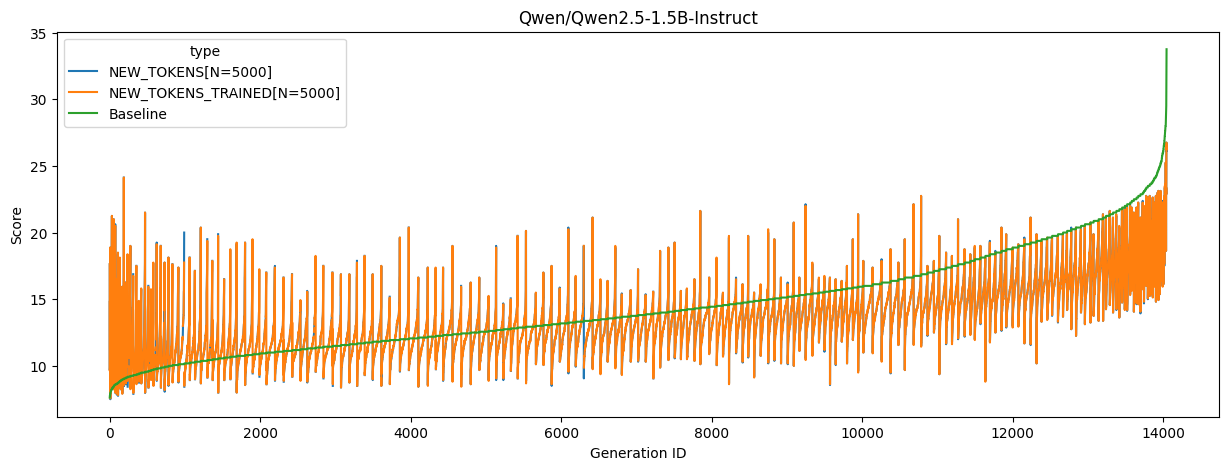
\includegraphics[width=\textwidth]{Figures/Appendix/token-rank-comparison_5000_qwen.png}
    \caption{Score comparison between original sub-token sequences and newly introduced tokens. Higher ranks indicate higher model preference.}
    \label{fig:new_token_rank:5000_qwen}
\end{figure}
\FloatBarrier
% ---------------------------------------------

\subsubsection*{Number New Tokens = 7500}
\begin{figure}[H]
    \centering
    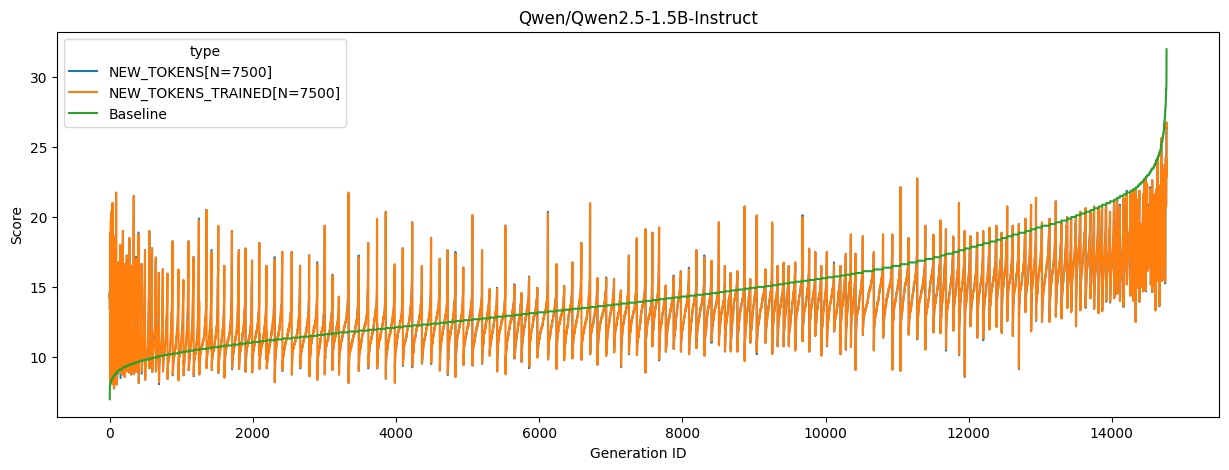
\includegraphics[width=\textwidth]{Figures/Appendix/token-rank-comparison_7500_qwen.png}
    \caption{Score comparison between original sub-token sequences and newly introduced tokens. Higher ranks indicate higher model preference.}
    \label{fig:new_token_rank:7500_qwen}
\end{figure}
\FloatBarrier
% ---------------------------------------------


% ======================================================================
\subsection*{Model \textit{HuggingFaceTB/SmolLM3-3B}}

% ---------------------------------------------
\subsubsection*{Number New Tokens = 1000}
\begin{figure}[H]
    \centering
    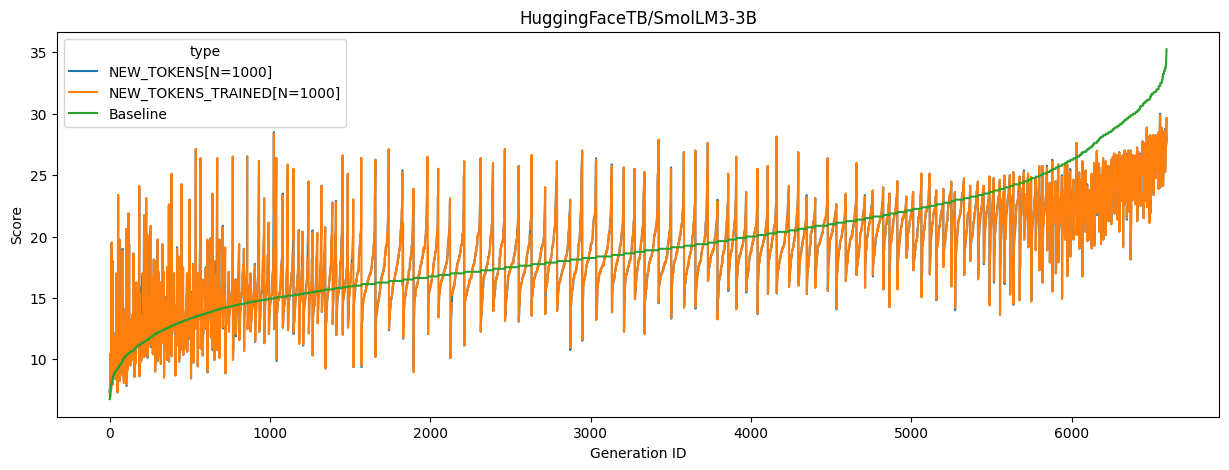
\includegraphics[width=\textwidth]{Figures/Appendix/token-rank-comparison_1000_smol3B.png}
    \caption{Score comparison between original sub-token sequences and newly introduced tokens. Higher ranks indicate higher model preference.}
    \label{fig:new_token_rank:1000_smol3B}
\end{figure}
\FloatBarrier
% ---------------------------------------------

\subsubsection*{Number New Tokens = 5000}
\begin{figure}[H]
    \centering
    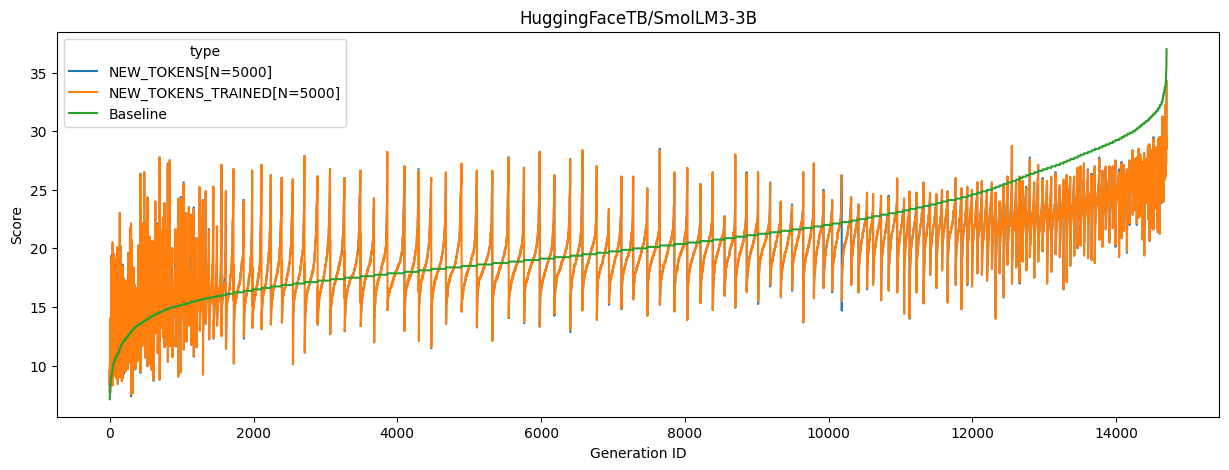
\includegraphics[width=\textwidth]{Figures/Appendix/token-rank-comparison_5000_smol3B.png}
    \caption{Score comparison between original sub-token sequences and newly introduced tokens. Higher ranks indicate higher model preference.}
    \label{fig:new_token_rank:5000_smol3B}
\end{figure}
\FloatBarrier
% ---------------------------------------------

\subsubsection*{Number New Tokens = 7500}
\begin{figure}[H]
    \centering
    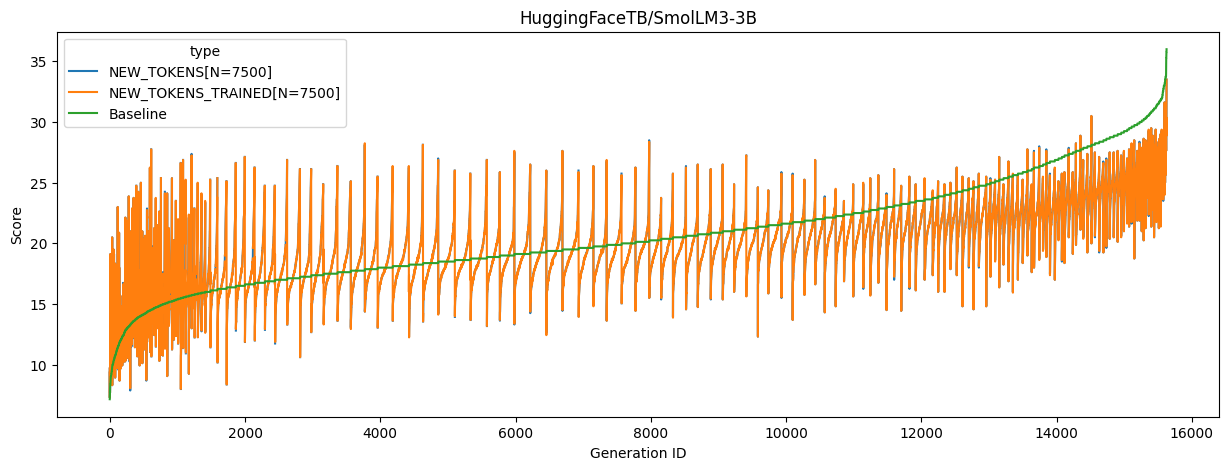
\includegraphics[width=\textwidth]{Figures/Appendix/token-rank-comparison_7500_smol3B.png}
    \caption{Score comparison between original sub-token sequences and newly introduced tokens. Higher ranks indicate higher model preference.}
    \label{fig:new_token_rank:7500_smol3B}
\end{figure}
\FloatBarrier
% ---------------------------------------------





% ======================================================================
% ======================================================================
% 
%
%                     Rank Diff Violin Distribution
%
%
% ======================================================================
% ======================================================================
\section*{Rank Differences Distribution}


% ---------------------------------------------
\subsection*{Model \textit{HuggingFaceTB/SmolLM2-135M}}
\begin{figure}[H]
    \centering
    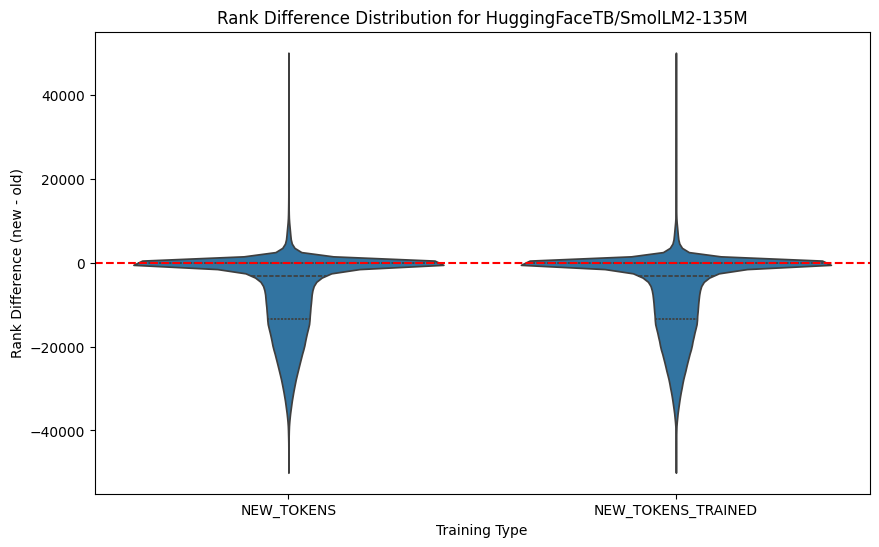
\includegraphics[width=1\textwidth]{Figures//Appendix/violin_smol135M.png}
    \caption{Distribution of rank differences across the entire results data. Negative numbers show preference towards \texttt{new\_token}.}
    \label{fig:violin_rank_dist:smol135M}
\end{figure}
% ---------------------------------------------


% ---------------------------------------------
\subsection*{Model \textit{Qwen/Qwen2.5-1.5B-Instruct}}
\begin{figure}[H]
    \centering
    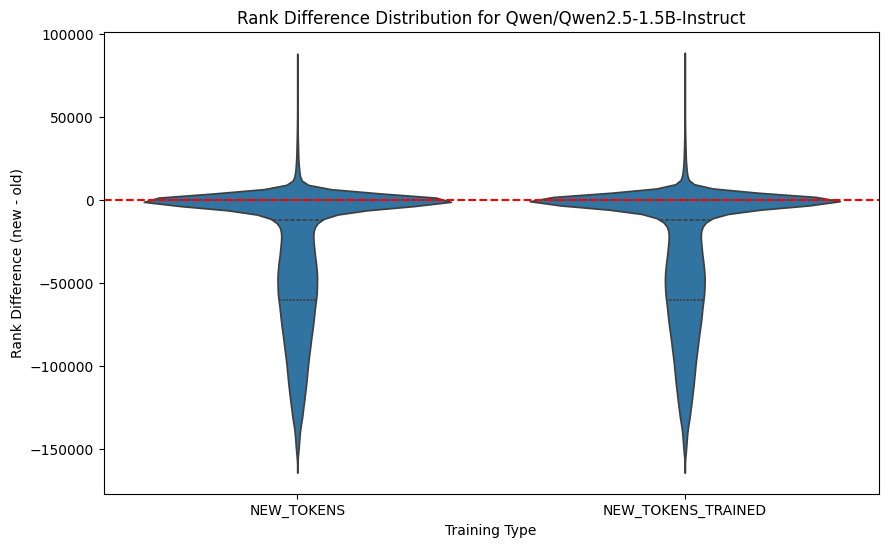
\includegraphics[width=1\textwidth]{Figures//Appendix/violin_qwen.png}
    \caption{Distribution of rank differences across the entire results data. Negative numbers show preference towards \texttt{new\_token}.}
    \label{fig:violin_rank_dist:qwen1.5B}
\end{figure}
% ---------------------------------------------


% ---------------------------------------------
\subsection*{Model \textit{HuggingFaceTB/SmolLM3-3B}}
\begin{figure}[H]
    \centering
    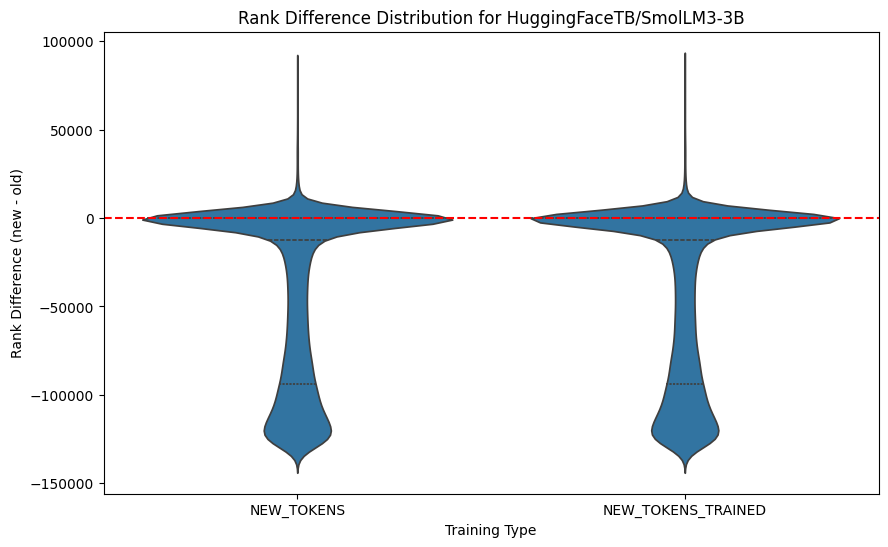
\includegraphics[width=1\textwidth]{Figures//Appendix/violin_smol3B.png}
    \caption{Distribution of rank differences across the entire results data. Negative numbers show preference towards \texttt{new\_token}.}
    \label{fig:violin_rank_dist:smol3B}
\end{figure}
% ---------------------------------------------
%\input{Appendices/AppendixB}
%\input{Appendices/AppendixC}

\backmatter


\end{document}
